
\section{Introduction} \label{sec:phases_introduction}

Energy efficiency has been one of the main focuses in computing nowadays, both in the mobile world and in high performance computing (HPC).
Indeed, it is essential to increase battery life and reduce heat generation, especially in HPC, where a small percentage of the savings energy can significantly reduce maintenance costs or environmental impact due to its scale of consumption.
For example, the leading Petaflop supercomputers consume in the range of 1 to 18 MW of electrical energy, with 1.5 MW on average, which we can estimate in millions of dollars in annual electricity cost \cite{Group2012HandbookSahni}. Furthermore, the International Energy Agency \cite{iea_2021} estimated that global data center electricity usage in 2020 was around 200-250 TWh, or around 1\% \cite{Corcoran2017EmergingICT} of global electricity demand  \cite{Mathew2012Energy-awareNetworks}.

Given the importance of this topic, modern desktops, cell phones, and HPC CPUs have built-in power management mechanisms.
That is because the processor is one of the main components that drain energy and can reach 50\% of the total system consumption \cite{Fan2007PowerComputer, Barroso2007TheComputing, Malladi2012TowardsDRAM}. Among the mechanisms implemented by the CPU, the most impactful and controllable via software are Dynamic Frequency and Voltage Scaling (DVFS), and Dynamic Power Management (DPM) ~\cite{Rotem2012Power-managementBridge, Brown2005ACPILinux, Hackenberg2015AnProcessor}.

DPM encompasses a set of techniques that take advantage of different energy levels in the system, such as active, inactive, and disabled~\cite{CARDOSO201717, Shuja2012Energy-efficientCenters, Benini2000AManagement}. The basic idea is to turn off devices and turn them on when needed. However, it is not a trivial task, and several variables need to be considered, such as the cost of switching, in terms of time and energy, how long it will remain in that state, the energy consumption in each state, and much more. This technique has the most significant gains when in systems where the static power is very high or where the system is idle for a long time. In such cases, some papers report energy savings of up to 70\%~\cite{Shuja2012Energy-efficientCenters, Benini2000AManagement}.

DVFS, on the other hand, allows real-time frequency and voltage control, depending on needs. This method is motivated by the fact that we can approximate the relationship of frequency to power as a cubic equation and frequency and performance as a linear equation \cite{Dayarathna2016DataSurvey, Group2012HandbookSahni}, implying that a reduction in frequency has a cubic impact on power and linear performance. However, it is not so simple because lowering the frequency leads to longer execution time, increasing power consumption. Therefore, determining the best voltage and frequency to employ under all conditions is a daunting task.

Although there are many studies on this topic, most works focus on implementing different optimization algorithms based on workload, and few studies pay attention to phase division, i.e. splitting the application in time intervals. Instead, most studies use static phase division to simplify the optimization math and compensate by implementing lightweight algorithms. However, this leads to a sub-optimization, as another phase division could result in different frequency values. In addition, there is an overhead associated with the moment the algorithm takes action that could be reduced if we knew the ideal moment for it to take action, making it possible even to allow heavier algorithms.

Therefore, this work proposes a methodology to study the division of time (phases) and analyzing possible gains, this approach is better justified in \cref{sec:proposed_approach}

The main contributions of this work are:
\begin{itemize}
	\item Heuristic algorithm for phase division
	\item Phase division optimization method
	\item Ideal number of phases for HPC applications
\end{itemize}
The proposed algorithm for phase division can be integrated in DVFS and DPM solutions to further improve them and archive better energy savings, described in \cref{sec:phase_division_algorithm}.

The phase optimization method can be used as an alternative for DVFS and DPM in energy saving optimization and also helps in the understanding of ideal phase division for a group of applications this is further detailed in \cref{sec:phases_optimization}.

The ideal number of phases is discussed in the results in \cref{sec:results} as well a comparison of the proposed phase optimization gains with the default method in Linux.

The conclusion of this work and proposed improvements are found in \cref{sec:conclusion}.

\section{Related work} \label{sec:phases_related_work}

One of the reference works in scheduling algorithms is the work of Irani et al. \cite{Irani2007}, where they formalized the problem of scheduling incoming jobs in a way that minimizes the total energy used, so that each job is completed after its arrival time and before its deadline. Although each problem has been considered separately, this was the first theoretical analysis of systems that could use both mechanisms.

Previous work has also used feedback-based approaches, as in Poellabauer et al. \cite{Poellabauer2005}, where past CPU behavior when running the application is used to predict future  CPU  requirements. However, mispredictions in these approaches can lead to missed deadlines,  sub-optimal energy savings,  or significant overheads due to frequent changes in the chosen frequency or voltage. One shortcoming of previous approaches is that they ignore other "indicators" of future CPU requirements, such as the frequency of I/O operations, memory accesses, or interrupts.

The thesis work of Saha et al. \cite{Saha2012} shows the timeliness and power consumption behavior of fourteen RT-DVFS schedulers through implementation and actual measurements. The schedulers include Static Earliest Deadline First (Static-EDF), Cycle Conserving Earliest Deadline First(CC-EDF), Look-Ahead Earliest Deadline First (LA-EDF), Snowdon-minimum (Snowdon-min), Resource-constrained Energy-Efficient Utility Accrual Algorithm (REUA), DynamicReclaiming Algorithm (DRA) and Aggressive Speed Reduction Algorithm(AGR) among others. They draw attention to the fact that most of the evaluations were based on simulations, which can mislead some results. Broadly, RT-DVFS techniques have two objectives: (i) Reduce energy consumption through DVFS, and (ii) Optimize task timeliness behavior through real-time resource management (deadline).

Pietri et al. \cite{Pietri2014} used slack reclamation to achieve energy savings. The goal is to exploit the idle slots of the processors that occurred due to the earlier completion time of the tasks compared with the latest finish time, which is constrained by deadline or data dependencies. In their model, the user submits a workflow for execution specifying a deadline for completion of the execution.

Mashayekhy et al. \cite{Mashayekhy2014} proposed a greedy algorithm, called Energy-aware  MapReduce  Scheduling  Algorithm  (EMRSA), that finds the assignments of the map and reduces tasks to the machine slots in order to minimize the energy consumed when executing the application. They consider an extensive data application consisting of a set of map and reduce tasks that need to be completed by deadline D.

Yousefi et al. \cite{Yousefi2018} present a task-based greedy scheduling algorithm, TGSAVE. This algorithm selects a slot for each task to minimize the total energy consumption of the MapReduce job for big data applications in heterogeneous environments without significant performance loss while satisfying the service level agreement (SLA). TGSAVE  finds solutions under deadlines up to 74\% tighter than the tightest one feasible by EMRSA, and it can meet deadlines as tight as only 12\%, on average, more significant than the makespan algorithm.

Crown scheduling is a static scheduling approach for sets of parallelizable tasks with a common deadline. Crown schedules are robust, i.e., the runtime prolongation of one task by a moderate percentage does not cause a deadline transgression by the same fraction. In addition, by speeding up some tasks scheduled after the lengthy task, the deadline can still be met at moderate additional energy consumption. In the work of Kessler et al. \cite{Kessler2021} they present a heuristic to perform this re-scaling online and explore the trade-off between additional energy consumption in normal execution and limitation of deadline transgression in delay cases.


In the work of \cite{Ajmal2021}, a green cloud computing algorithm named "Cost-based Energy Efficient Scheduling Technique for Dynamic Voltage Frequency Scaling (DVFS) Systems (CEEST)" is proposed. The proposed algorithm reduces energy consumption without compromising the quality of service (QoS). This algorithm aims to optimize and manage servers in the datacenters by utilizing maximum resources and powering off the underutilized servers. Furthermore, CEEST utilizes the scaling of virtual machines to finish jobs within the deadlines to reduce violations of service level agreement (SLA). 

All of these works at some point considered a deadline (defined by the user or the system) that defines the phases of the job; this means that choosing a different deadline could result in completely different energy savings. In our paper, we study the impact of this phase division on the application's energy consumption. In this context, we estimate how much energy could be saved if an algorithm could magically give the ideal deadline.

Although most of the works consider the deadline, some works also take job division as part of the optimization problem. In the paper of Agrawal et al. \cite{Agrawal2021}, they show that if the jobs can be divided into arbitrary parts, the minimum-energy schedule can be generated in linear time, giving exact scheduling algorithms. For the cases where jobs are non-divisible, they claimed a proof that the scheduling problems are NP-hard, while giving approximation algorithms for these with their bounds.
In this case, where no deadline is defined, the phase division is indirectly considered by solving the optimization problem of minimizing the energy. The problem, in this case, is that several constraints restrict the optimization problem while our approach works with measured data, meaning that we can find solutions independent of the constraints.

\section{Proposed approach} \label{sec:proposed_approach}
To find the optimal phase division, we would have to ensure that the one we choose is the most energy-efficient among all possible divisions and different combinations of power configurations.
This mathematical problem can be modeled in many ways, but always with some concessions to make it solvable. Another option would be by brute force, but there are infinite possibilities for splitting phases, although some hardware limitations make our analysis more accessible. With that in mind, we decided to create a heuristic that comes the closest to brute force using hardware limitations to make it viable.

The first limitation is that the processor has a limited speed at which it can act. In other words, a division that can act would make no sense, limiting our analysis to discrete-time intervals at the processor's maximum performance speed.

This already limits our exploration space a lot, but even so, it is still unfeasible. For example, considering $d_t$ as the minimum processor action interval, $T$ the total application time, and $C$ the number of power settings. The number of possibilities could be estimated by:
$ \left(\frac{T}{d_t}\right)^C.$
This number grows astronomically because $d_t$ is in a time range of microseconds, $T$ seconds or minutes, and C of hundreds. To give an idea, we can estimate this number to be in a range of $10^{7000}$.

Another thing that we can see is that each configuration gives the power profile for a given application, and phase division is just a combination of these configurations. This allows us to reduce further our exploration of space. For example, if we ran each power setting once and we had a way of combining them, our problem now would be feasible. To make this possible, we assume that the configuration change only affects the program speed and that the power consumption is independent of the previous settings.


This approach aims to bring the best of both worlds. We want simulation speed but with actual measurement data for greater accuracy. Our algorithm runs with measured data from a real system. The idea is to run the application with all possible configurations (e.g., frequency and number of active cores) of the machine without time division and estimate power consumption for different phase divisions.

\section{Phase division algorithm} \label{sec:phase_division_algorithm}
To analyze the impact of configurations and identify the optimal phase division, we propose a zero-order integrator, which calculates the energy in an interval for a given configuration. The integrator uses the data gathering described in \cref{subsec:data_gathering}.

Figure \ref{fig:zero_order} shows an example energy computation for an application with four different power configurations. The phases are, first, defined in terms of the percentage of execution. Then, the integrator will run over each phase using the selected power profile obtained from the measurements, and accumulate the total energy consumption.

\begin{figure}[H]
	\centering
	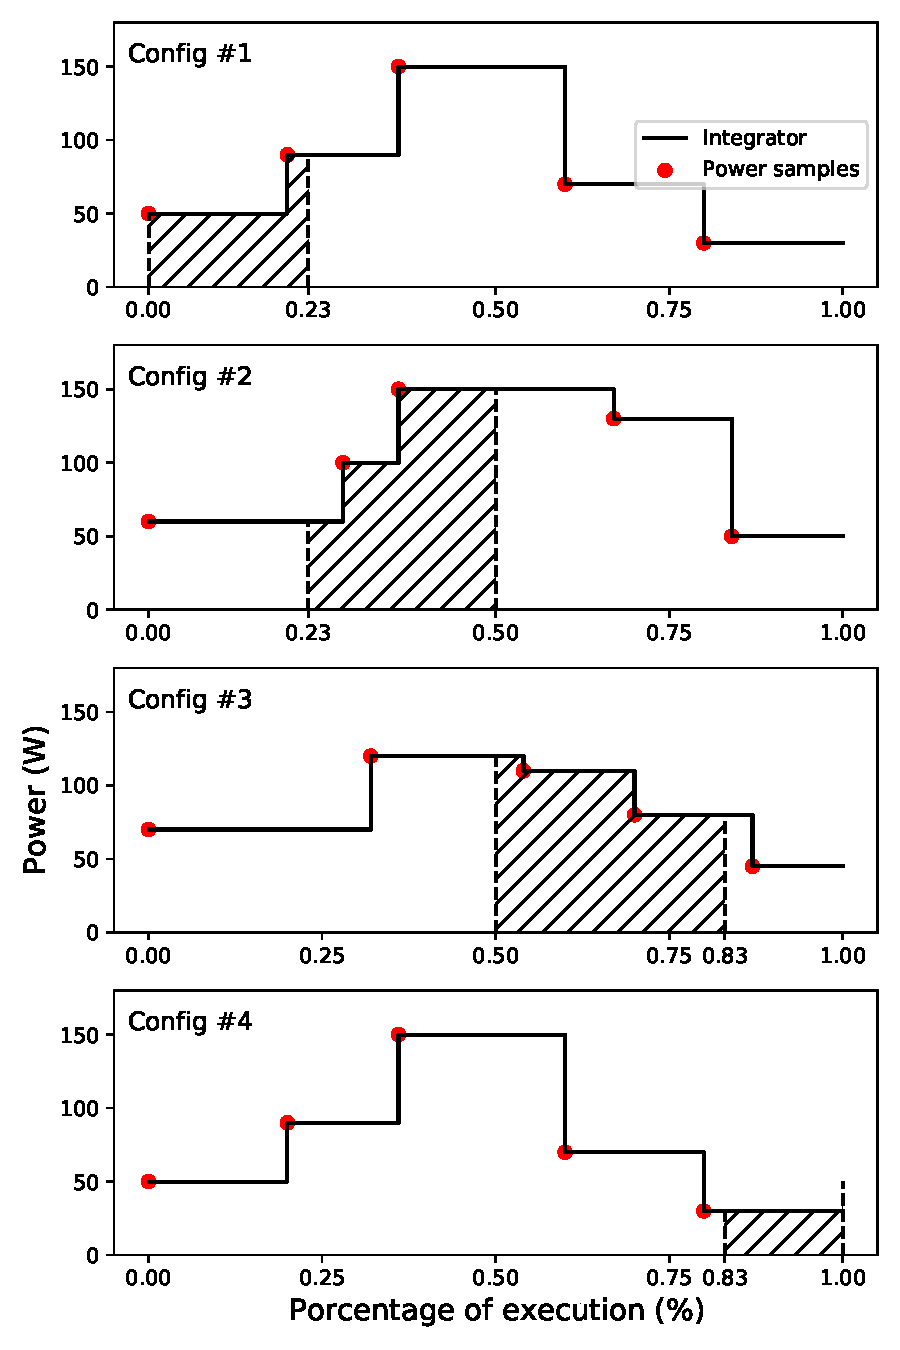
\includegraphics[width=\columnwidth]{phases/figures/integrator.pdf}
	\caption{Power vs percentage of execution for a given application in several configurations (1 to 4). For each configuration, the energy in each phase is represented by the hatched area.}
	\label{fig:zero_order}
\end{figure}

The pseudo-algorithm for the integrator is described below:

\begin{lstlisting}[language=c++]
	integrator(total_time, nsamples,
	times, powers
	begin_phase, end_phase)
	{
		energy = 0;
		ti = total_time * begin_phase; // initial time
		tf = total_time * end_phase; // final time
		
		idx_i = 0, idx_f = 0;
		
		// find the index of the first sample in the range
		for (idx_i= 0; idx_i<nsamples; idx_i++)
		if (times[idx_i] >= ti)
		break;
		idx_i = (idx_i != 0) ? idx_i - 1 : 0;
		
		// find the index of last sample in the range
		for (idx_f= idx_i; i<nsamples; idx_f++)
		if (times[idx_f] >= tf)
		break;
		idx_f = (idx_f != 0) ? idx_f - 1 : 0;
		
		// in case there is only one sample
		if (idx_i == idx_f) 
		return (tf-ti)*powers[idx_i];
		
		// handle the edges
		energy=(times[idx_i+1]-ti)*powers[idx_i]
		energy+=(tf-times[idx_f])*powers[idx_f];
		
		// handle samples in between
		for (int i= idx_i+1; i<idx_f; i++)
		energy += (times[i+1]-times[i])*powers[i];
		
		return energy;
	}
\end{lstlisting}

This algorithm works by...

\section{Phases optimization} \label{sec:phases_optimization}

\subsection{Data gathering} \label{subsec:_phases_data_gathering}

Using the Pascal framework \cite{electronics11050689}, the data was collected by running applications in all possible configurations. In this system, that is 32 cores and 13 frequencies, means a total of 416 (32*13) possible configurations per application. Power samples were taken from dedicated sensors in the IPMI system with a sample rate of 0.5 seconds.

\subsection{Phase optimization algorithm} \label{subsec:phase_optimization_algorithm}
To obtain an optimal energy configuration for a given phase division, we can run all possible configurations and select the one that leads to a minimal consumption, as shown in the pseudo-algorithm below:

\begin{lstlisting}
	phase_optimization(configs, phases)
	{
		total_en = 0;
		for (i = 0; i<phases.size(); i++)
		{
			min_en = -1;
			for (j = 0; j<configs.size(); j++)
			{
				en = integrator(
				configs[j].total_time, 
				configs[j].nsamples,
				configs[j].time_samples,
				configs[j].power_samples,
				phases[i], phases[i + 1]);
				if (min_en == -1 || en < min_en)
				{
					min_en = en;
					min_conf = configs[j];
				}
			}
			total_en += min_en;
		}
		return total_en;
	}
\end{lstlisting}

This method can now obtain an optimal energy configuration for a given phase. The next step is to find the best phase division.


\section{Results} \label{sec:results}
Now that we can evaluate phase divisions, we need to answer two questions, what is the best number of phases, and what is the best division within this number?
For that, we used the algorithm described previously in \cref{sec:heuristic} as the objective of a minimization problem where we want to find the vector of phases that minimizes the total energy. 
A genetic algorithm will be used as a solver, whose execution process can be accelerated by controlling the mutation and the initial population since some constraints are already known.
For instance, to study the phases in the range of 3 to 100 divisions, we use a GA with a population of $10^3$ individuals. We keep the best 10\% individuals from each generation, while having a 10\% of mutation rate, over 300 generations. The reproduction function for the GA combines half of the phases of one individual with another, and the mutation will randomly change one division.

We used the applications described in \cref{sec:casestudyapplication}, to compute the optimal phase selection. The \cref{fig:relative_energy} indicates, for each application, the energy consumption according to the number of phases, compared to an optimized single-phase.

\begin{figure}[H]
	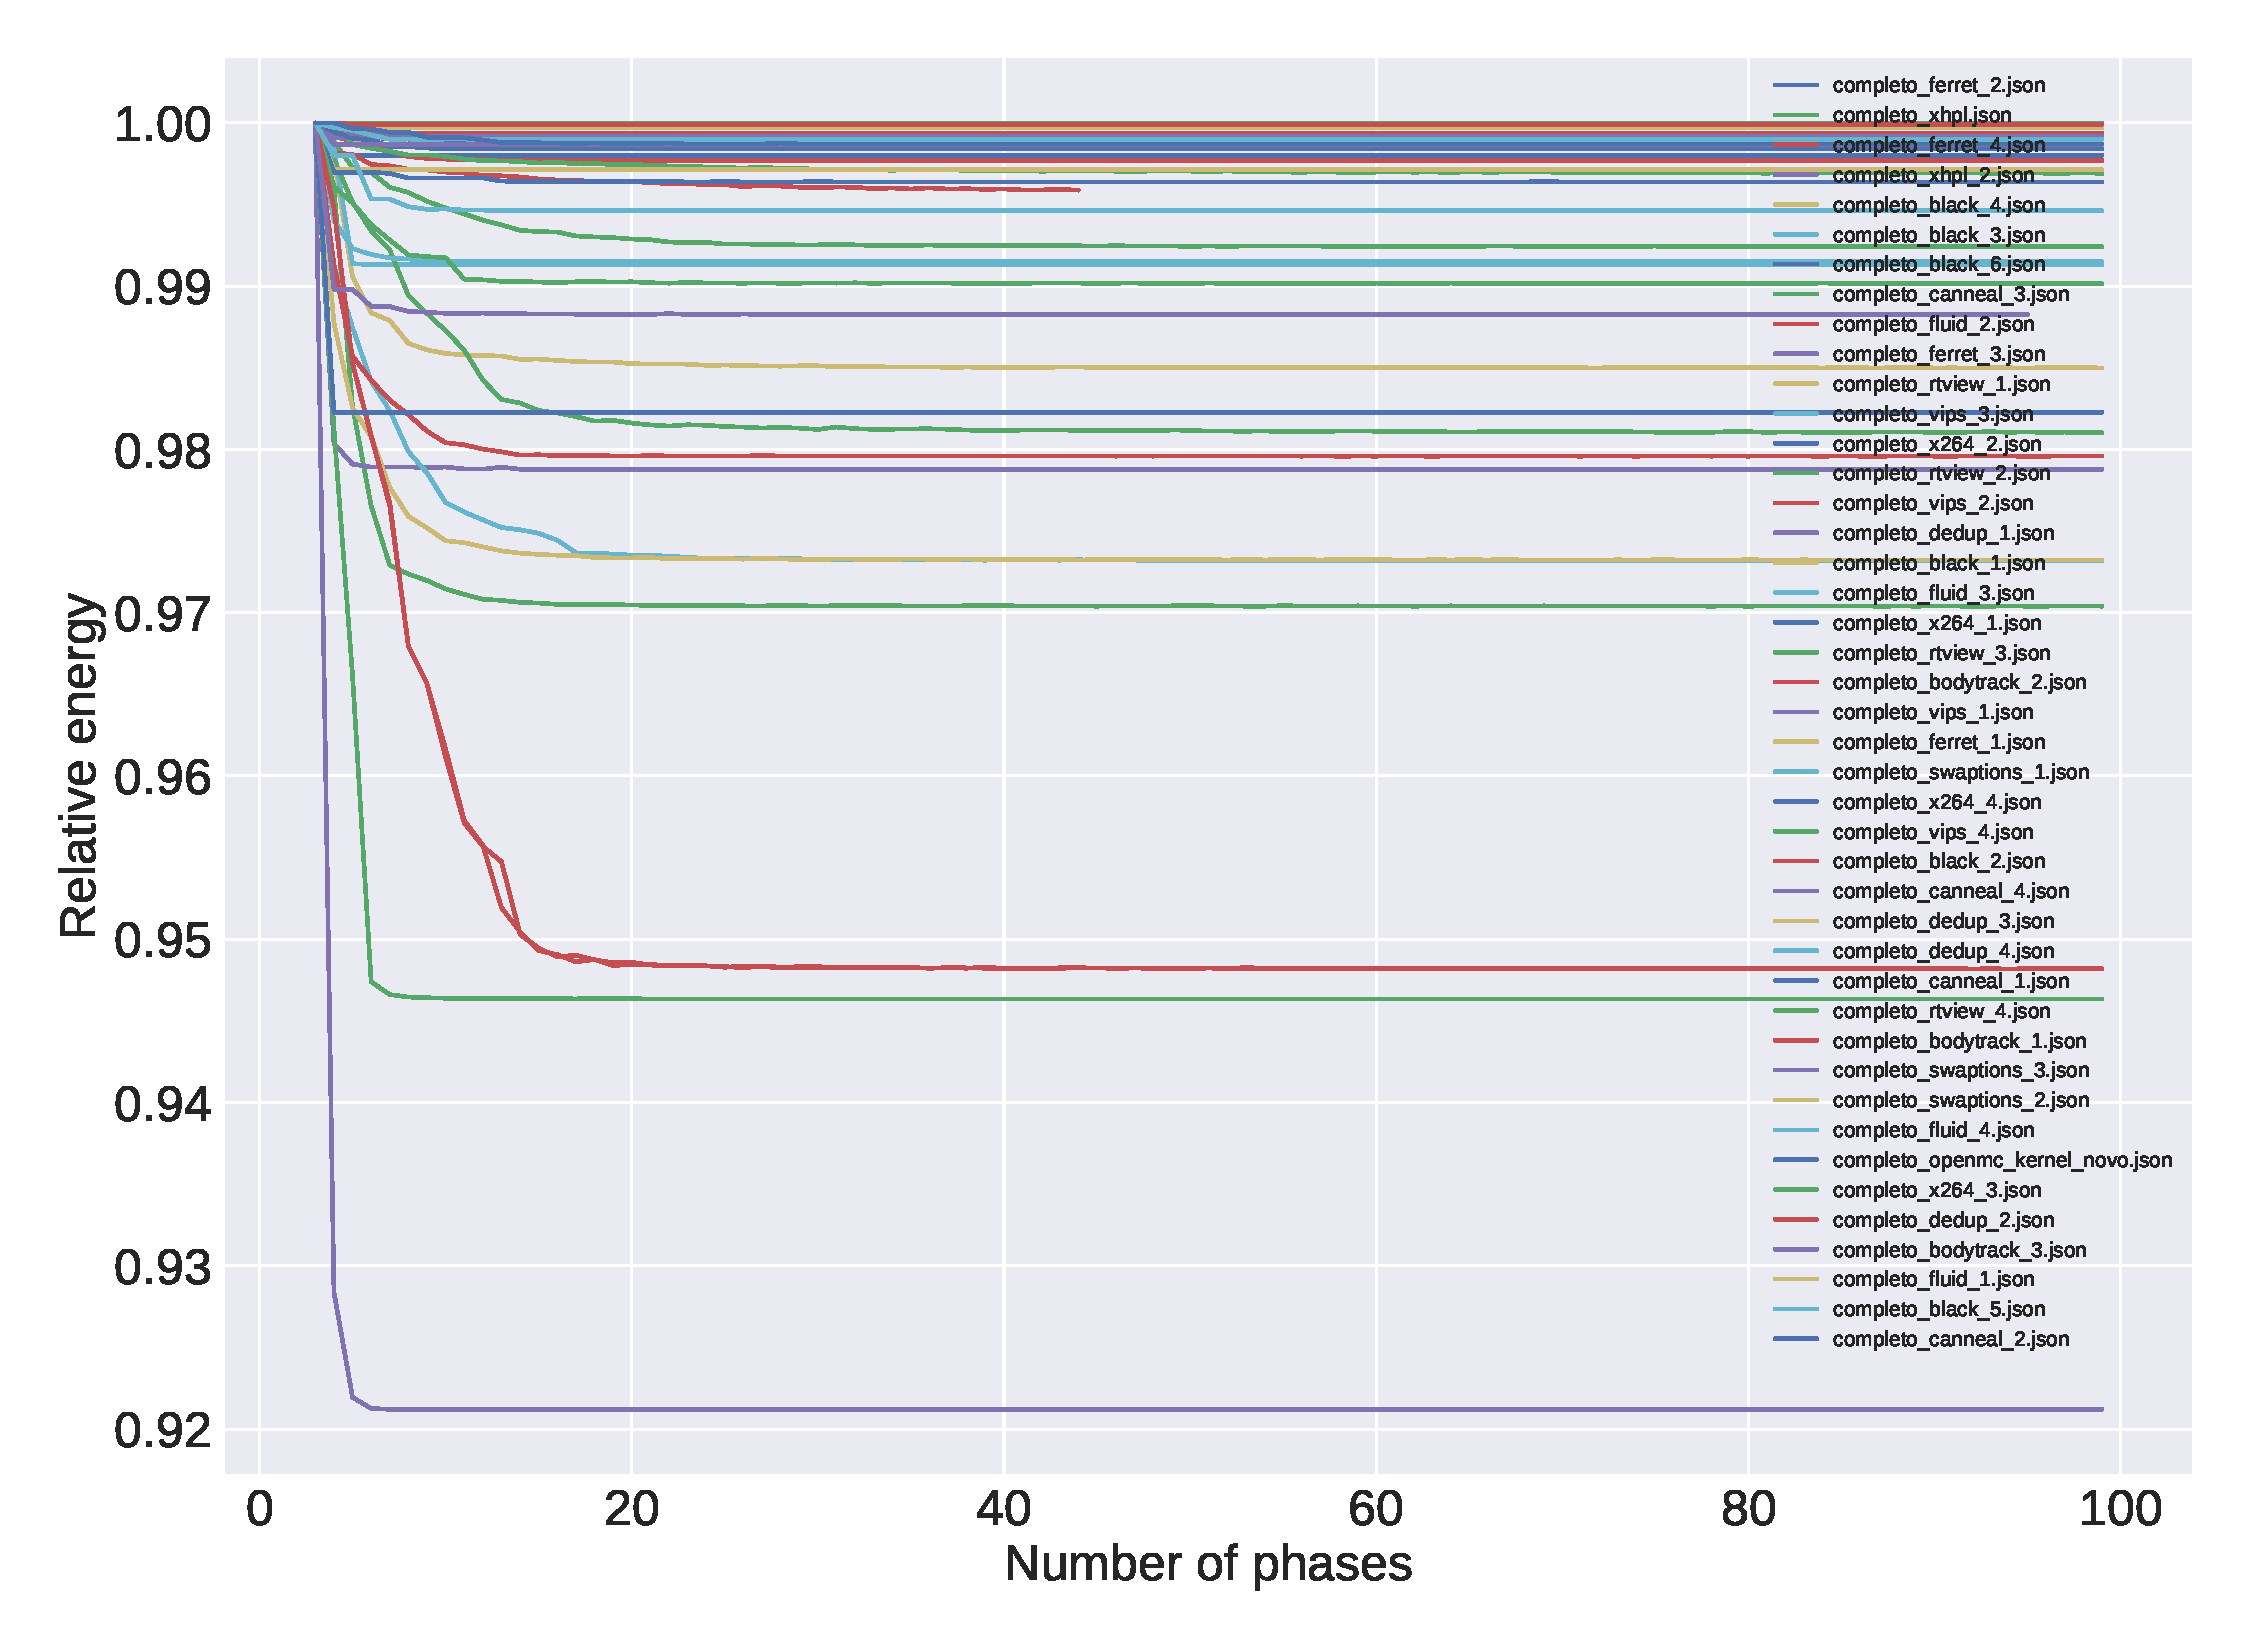
\includegraphics[width=\columnwidth]{fingerprint/figures/energy_per_phase.pdf}
	\caption{Relative energy (compared to the single-phase optimal configuration) vs number of phases using applications from PARSEC 3.0, HPC, and Openmc benchmarks with different sizes' inputs.}
	\label{fig:relative_energy}
\end{figure}

The \cref{fig:relative_energy} shows very interesting results. The energy consumption of the optimal single-phase configuration is always higher for all cases. Furthermore, it is not necessary to divide the application into more than 35 phases. Indeed, the energy gain is negligible beyond 35 phases.

The \cref{fig:hist_optimal_phase} shows in more detail the ideal number of phases for all of our tests, there we can see that most applications reach the ideal configuration with less than 20 phases, while there is still a uniform distribution to a higher number of phases.

\begin{figure}[H]
	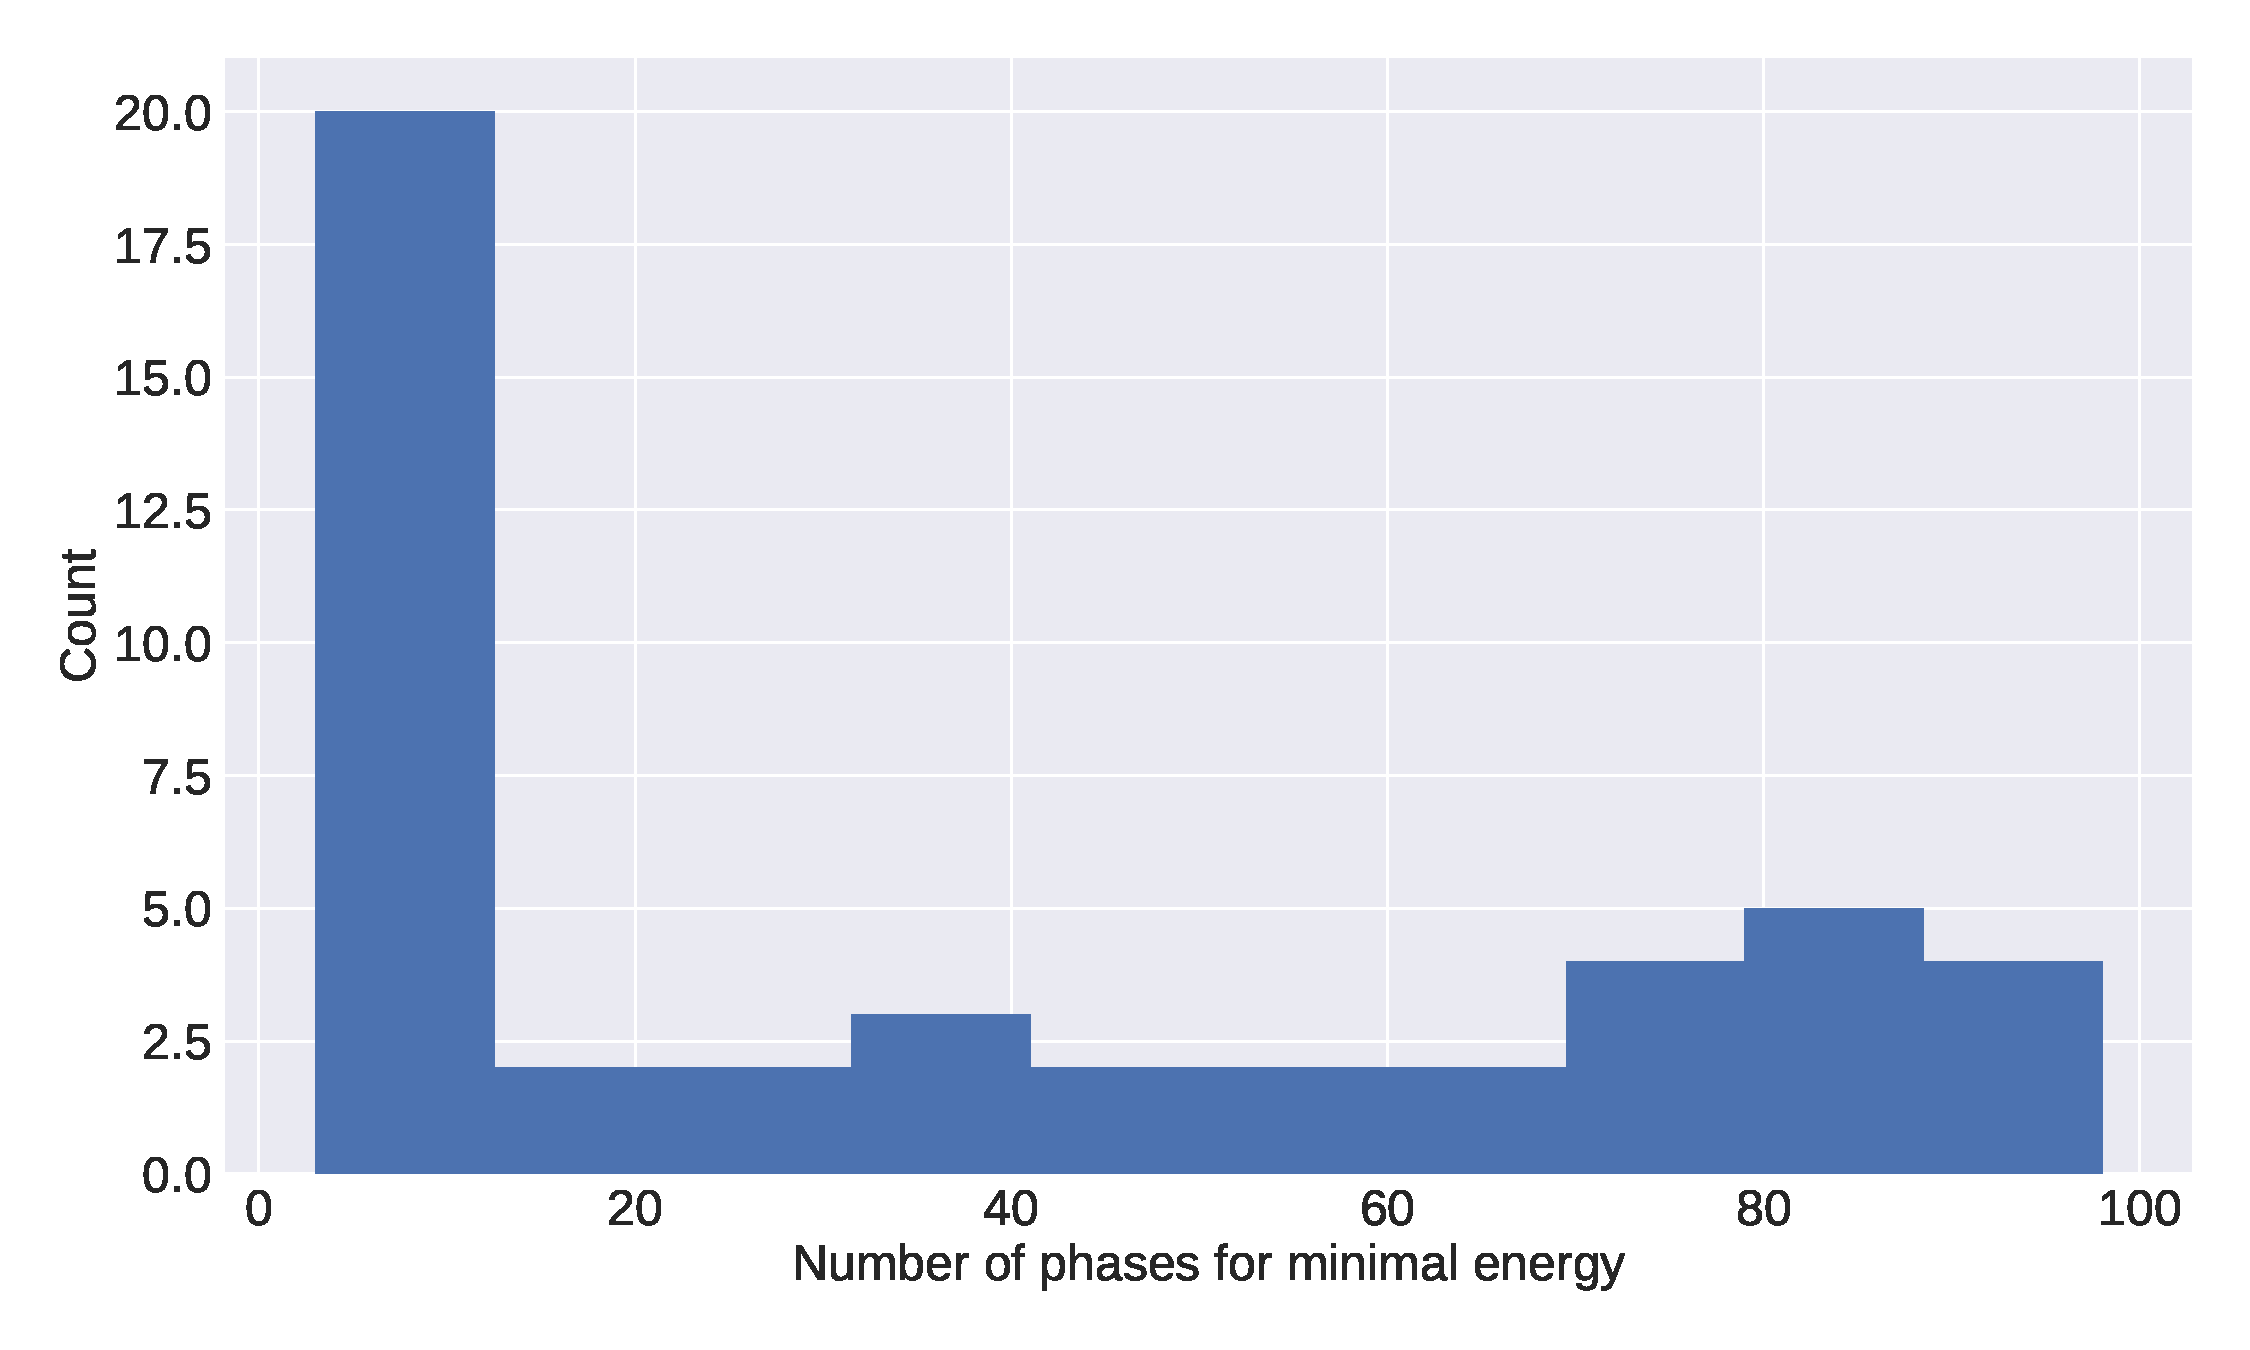
\includegraphics[width=\columnwidth]{phases/figures/min_phases_distribution.pdf}
	\caption{Histogram showing the frequency of the optimal number of phases for all applications}
	\label{fig:hist_optimal_phase}
\end{figure}

The results meet our expectation that the optimum of n-divisions phases will always be better than or equal to n-1 divisions. This becomes clearer when we look at the number of cores, in \cref{fig:cores_control_1} and \cref{fig:cores_control_2}, and frequencies, in  \cref{fig:black_control_1} and \cref{fig:black_control_2} for two particular applications, Bodytrack and Blackscholes. These applications demonstrate the optimal frequency and cores do not fundamentally change between 35 and 99 phases.
%Since starting from a certain number of divisions does not change the control signals since dividing an ideal phase into two would result in two phases with the same control signals. Therefore, the energy will remain the same, and there is no reason to increase the number of phases beyond that.

\begin{figure}[h]
	\centering
	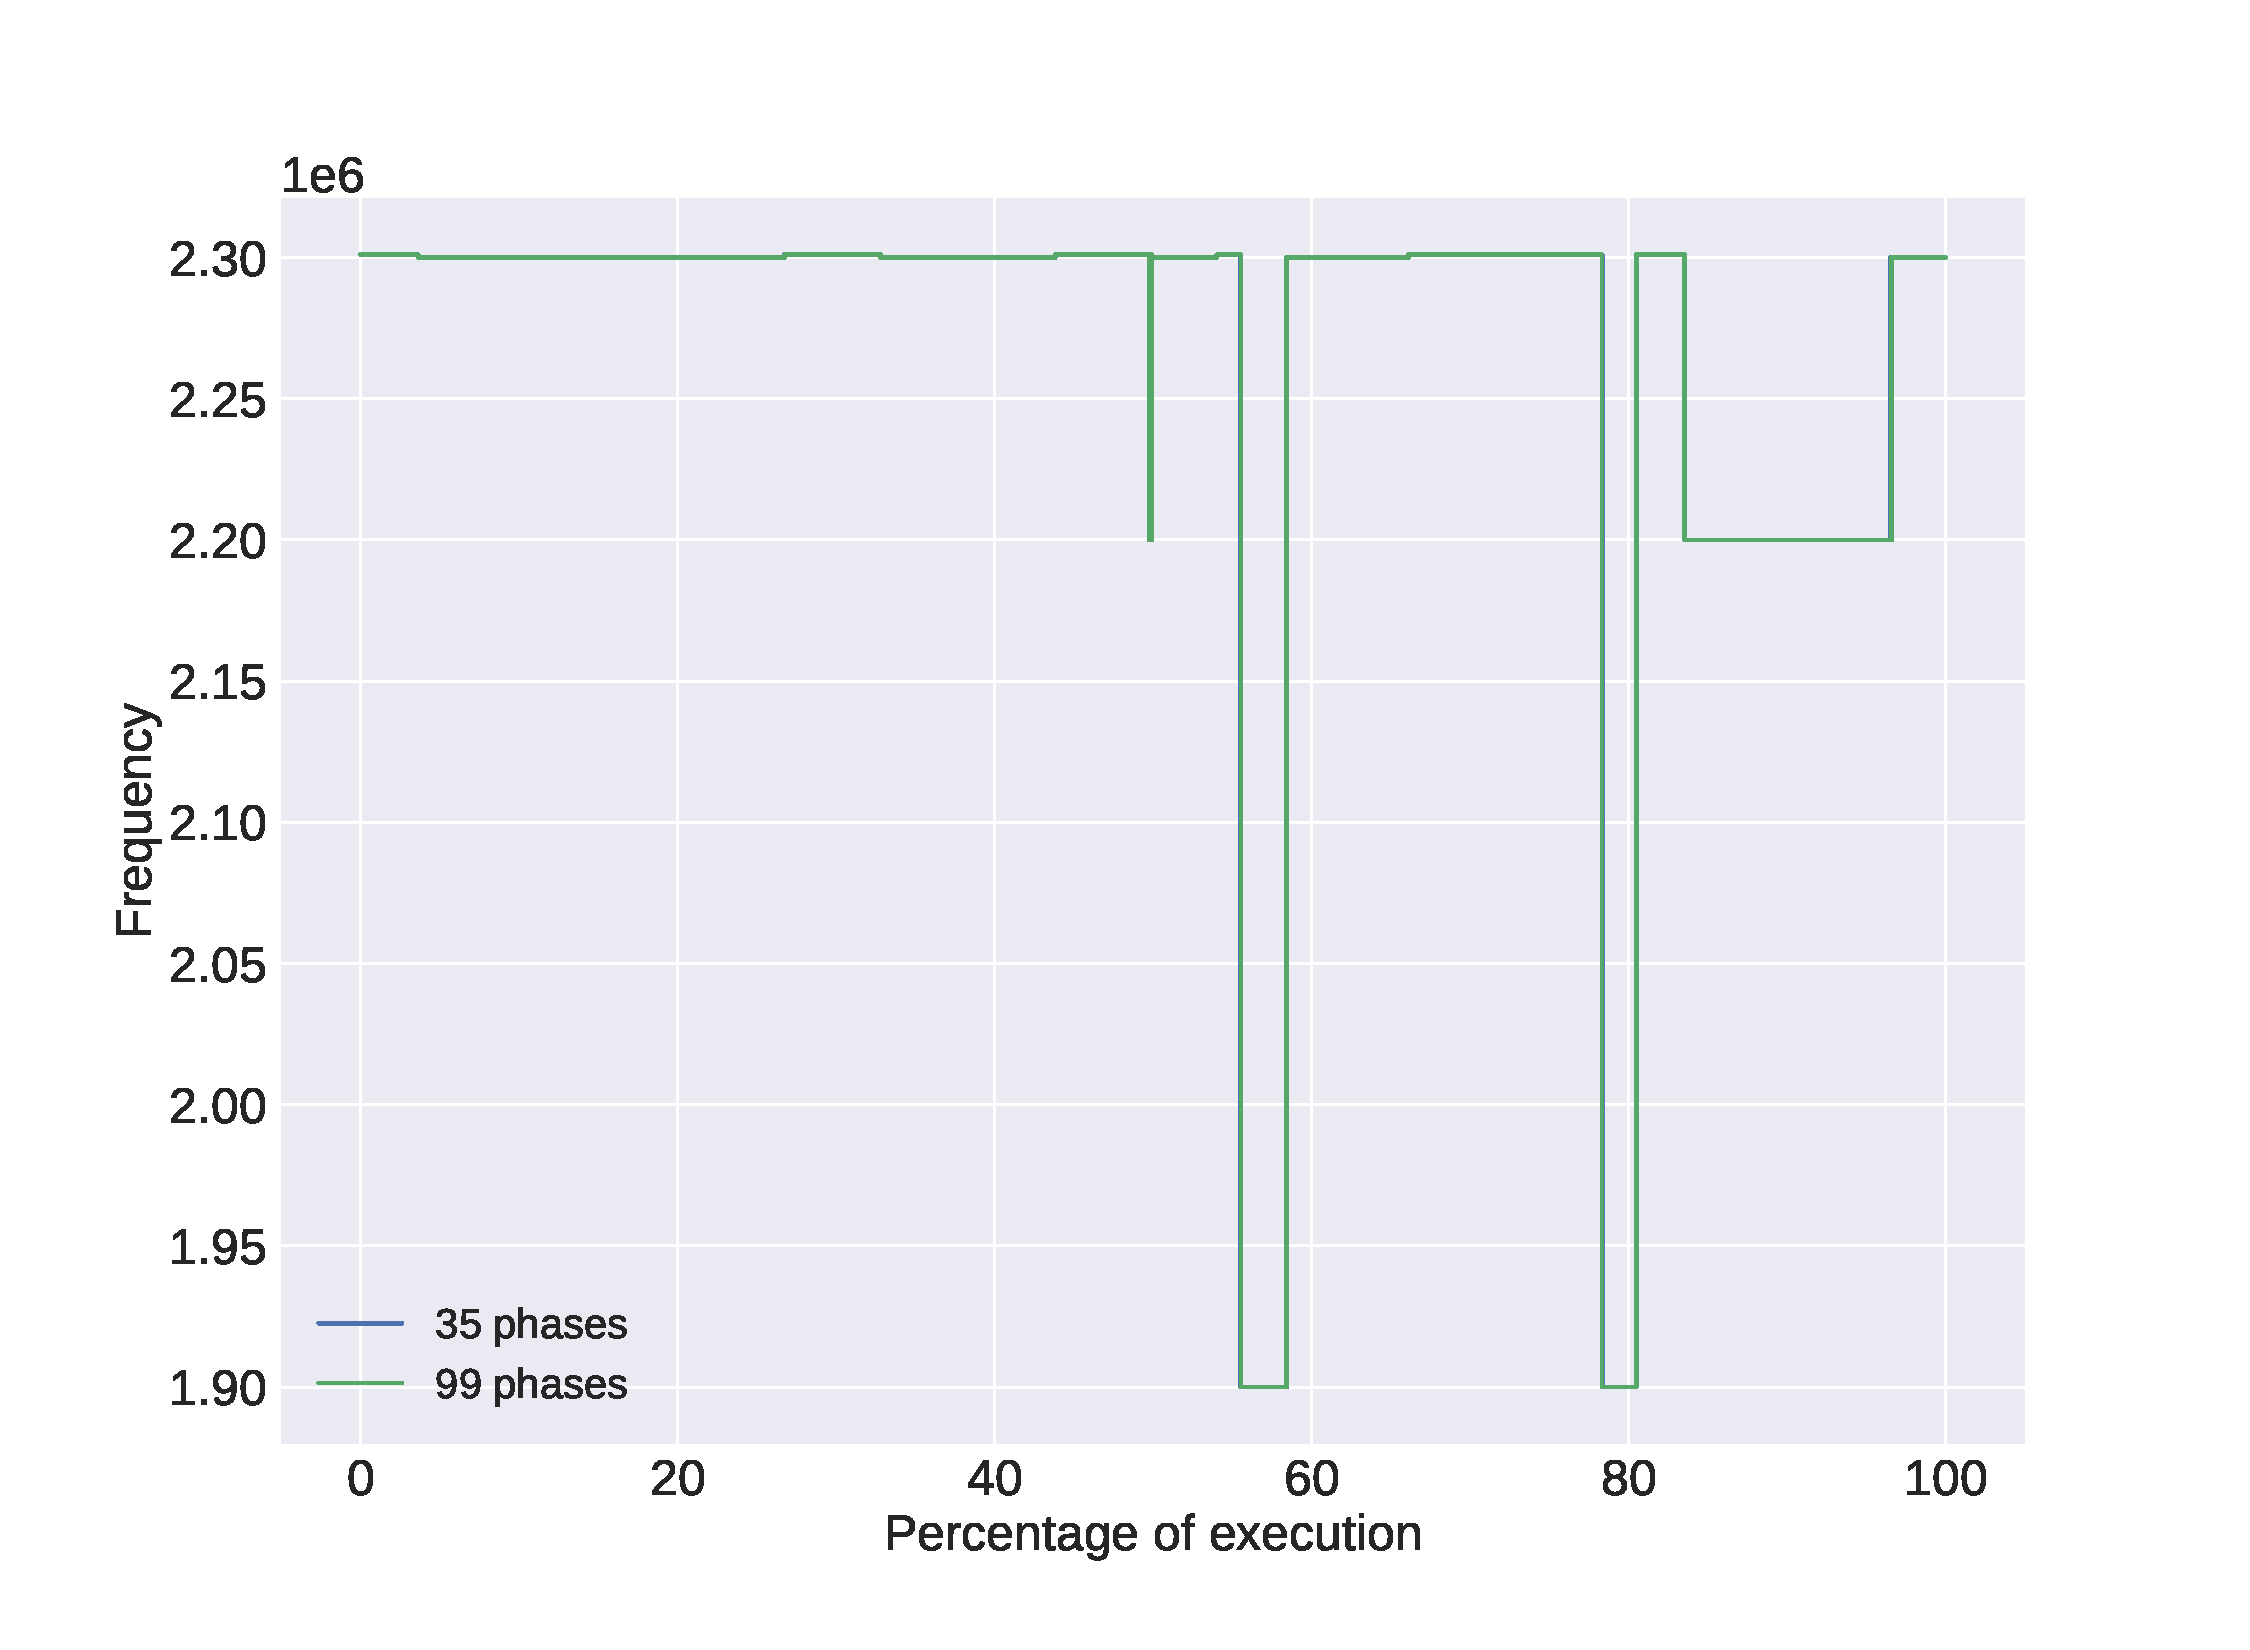
\includegraphics[width=\columnwidth]{phases/figures/signals/completo_bodytrack_1_freq_signals_cmp.pdf}
	\caption{execution frequency vs percentage of execution for the Bodytrack application, comparison when using 35 and 99 phases.}
	\label{fig:black_control_1}
\end{figure}%

\begin{figure}[h]
	\centering
	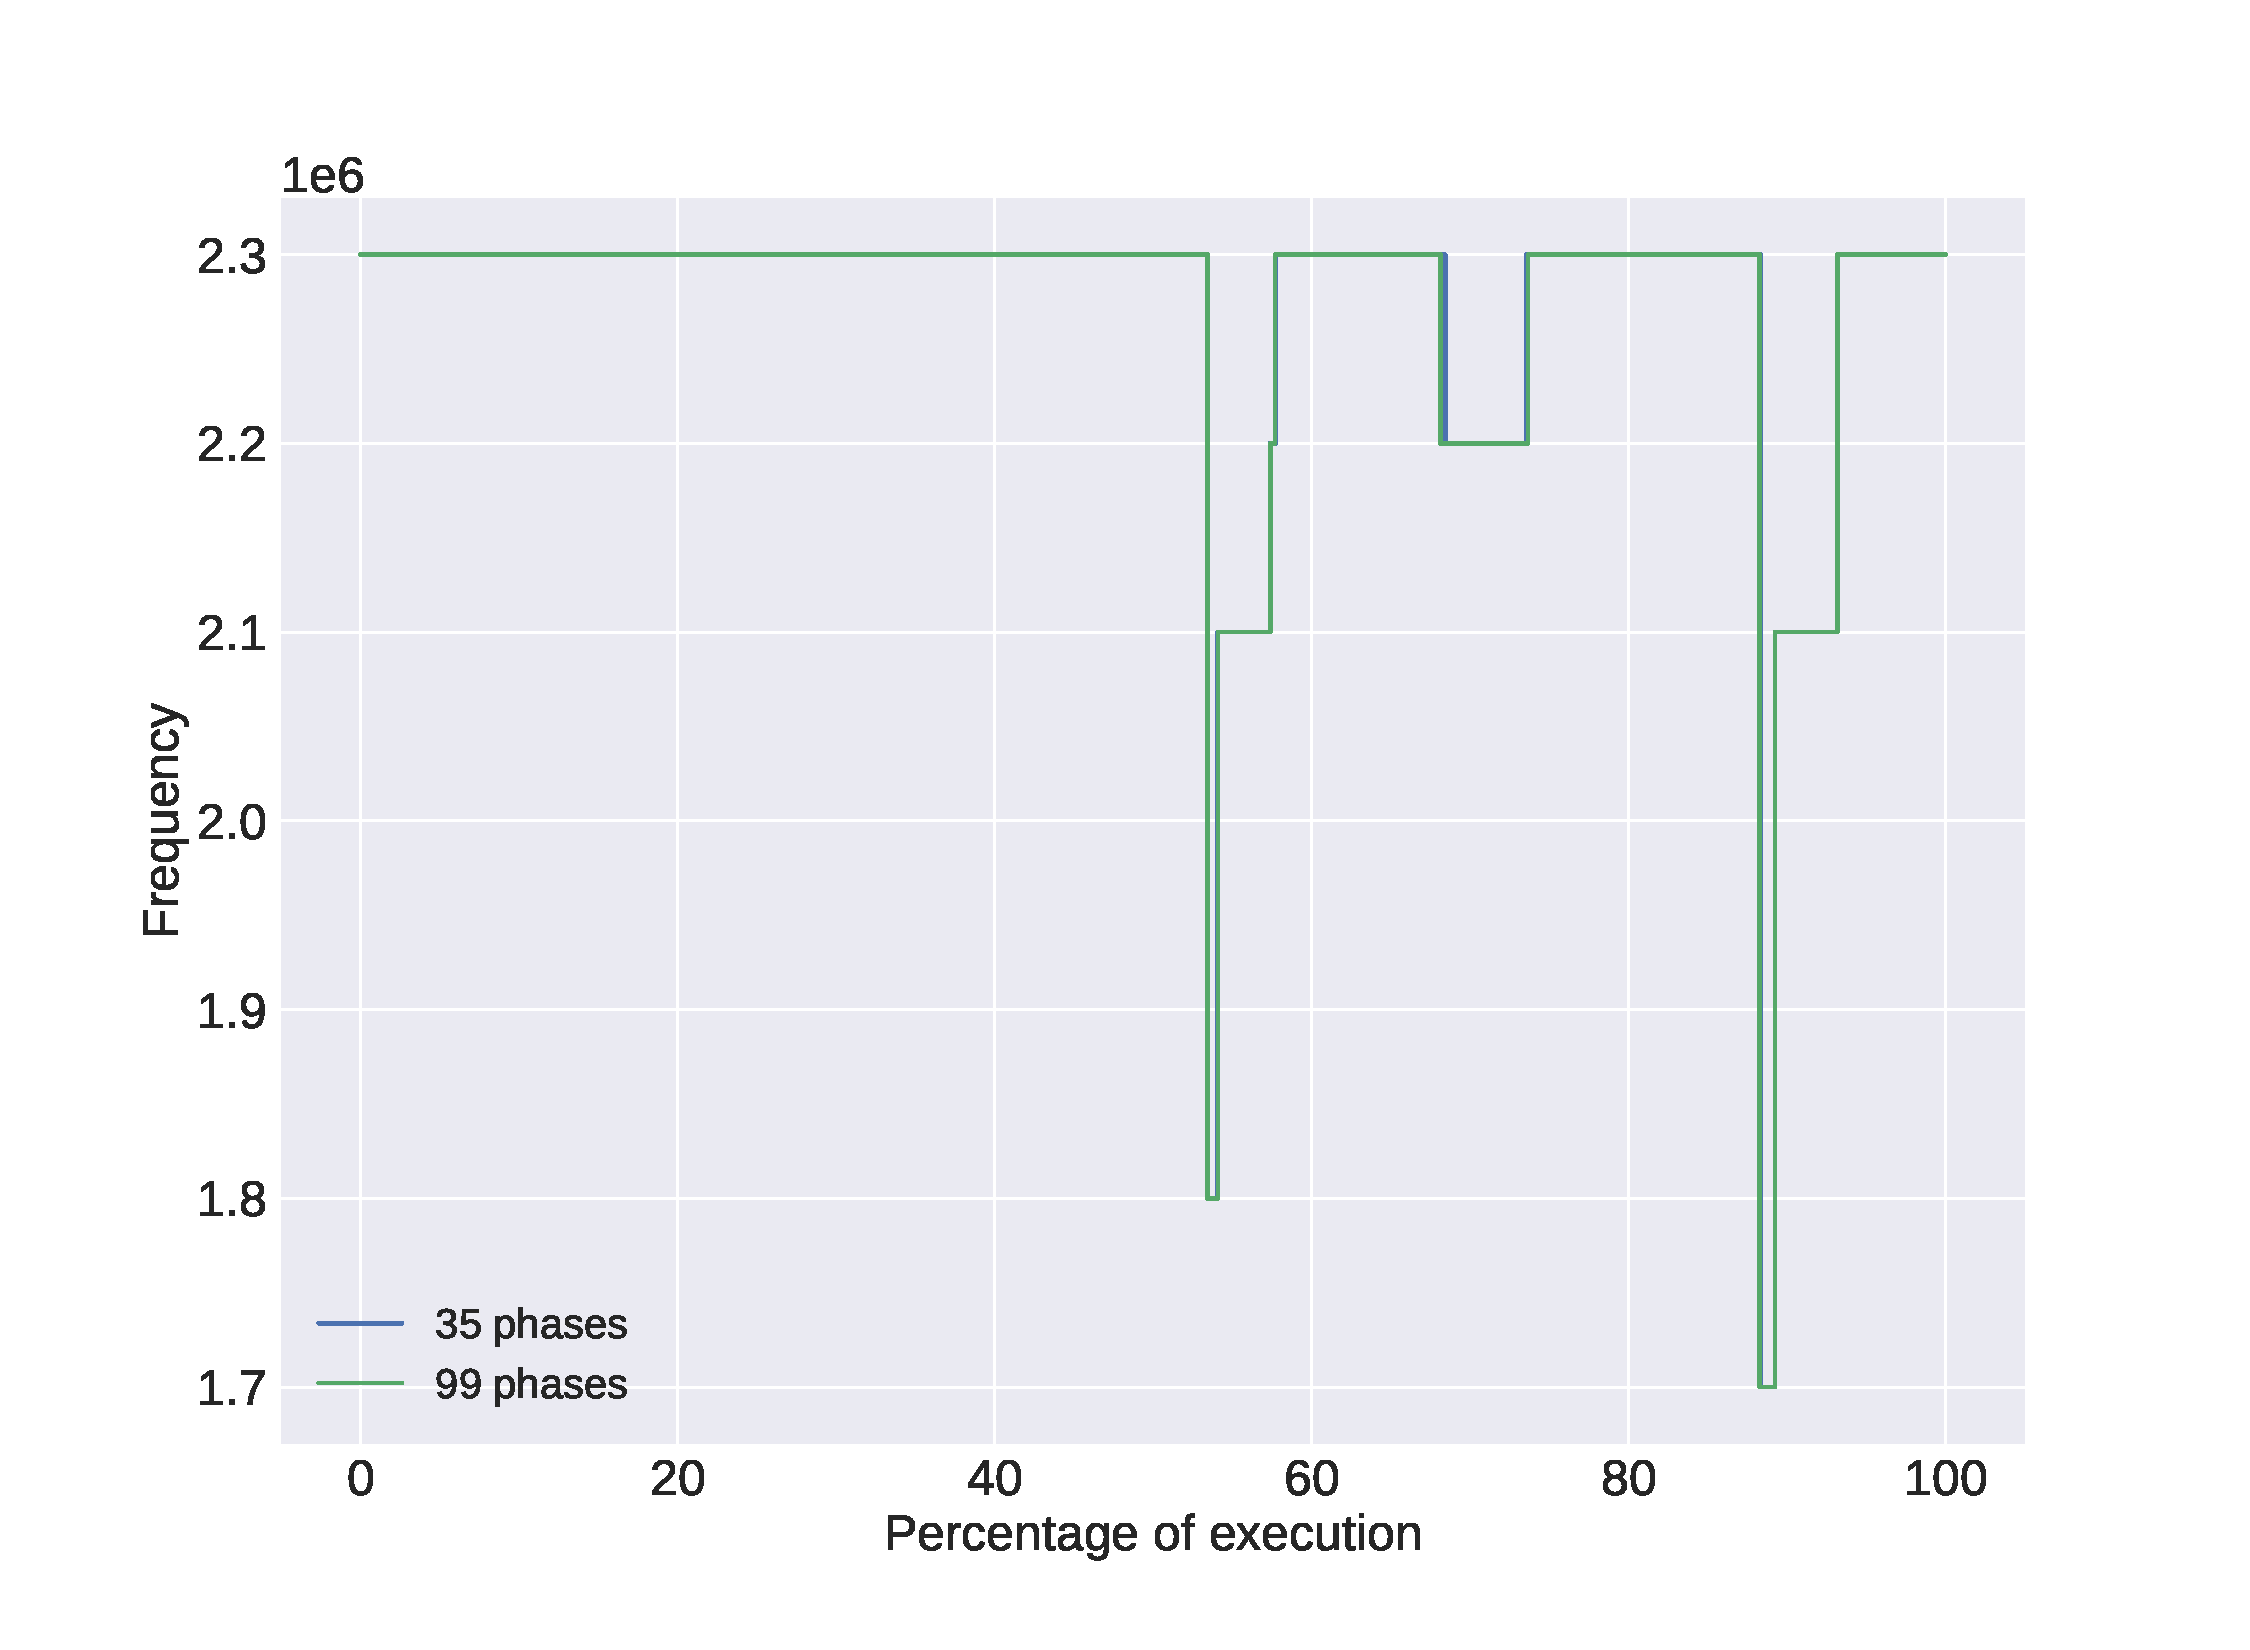
\includegraphics[width=\columnwidth]{phases/figures/signals/completo_black_1_freq_signals_cmp.pdf}
	\caption{execution frequency vs percentage of execution for the Blackscholes application, comparison when using 35 and 99 phases.}
	\label{fig:black_control_2}
\end{figure}%

\begin{figure}[h]
	\centering
	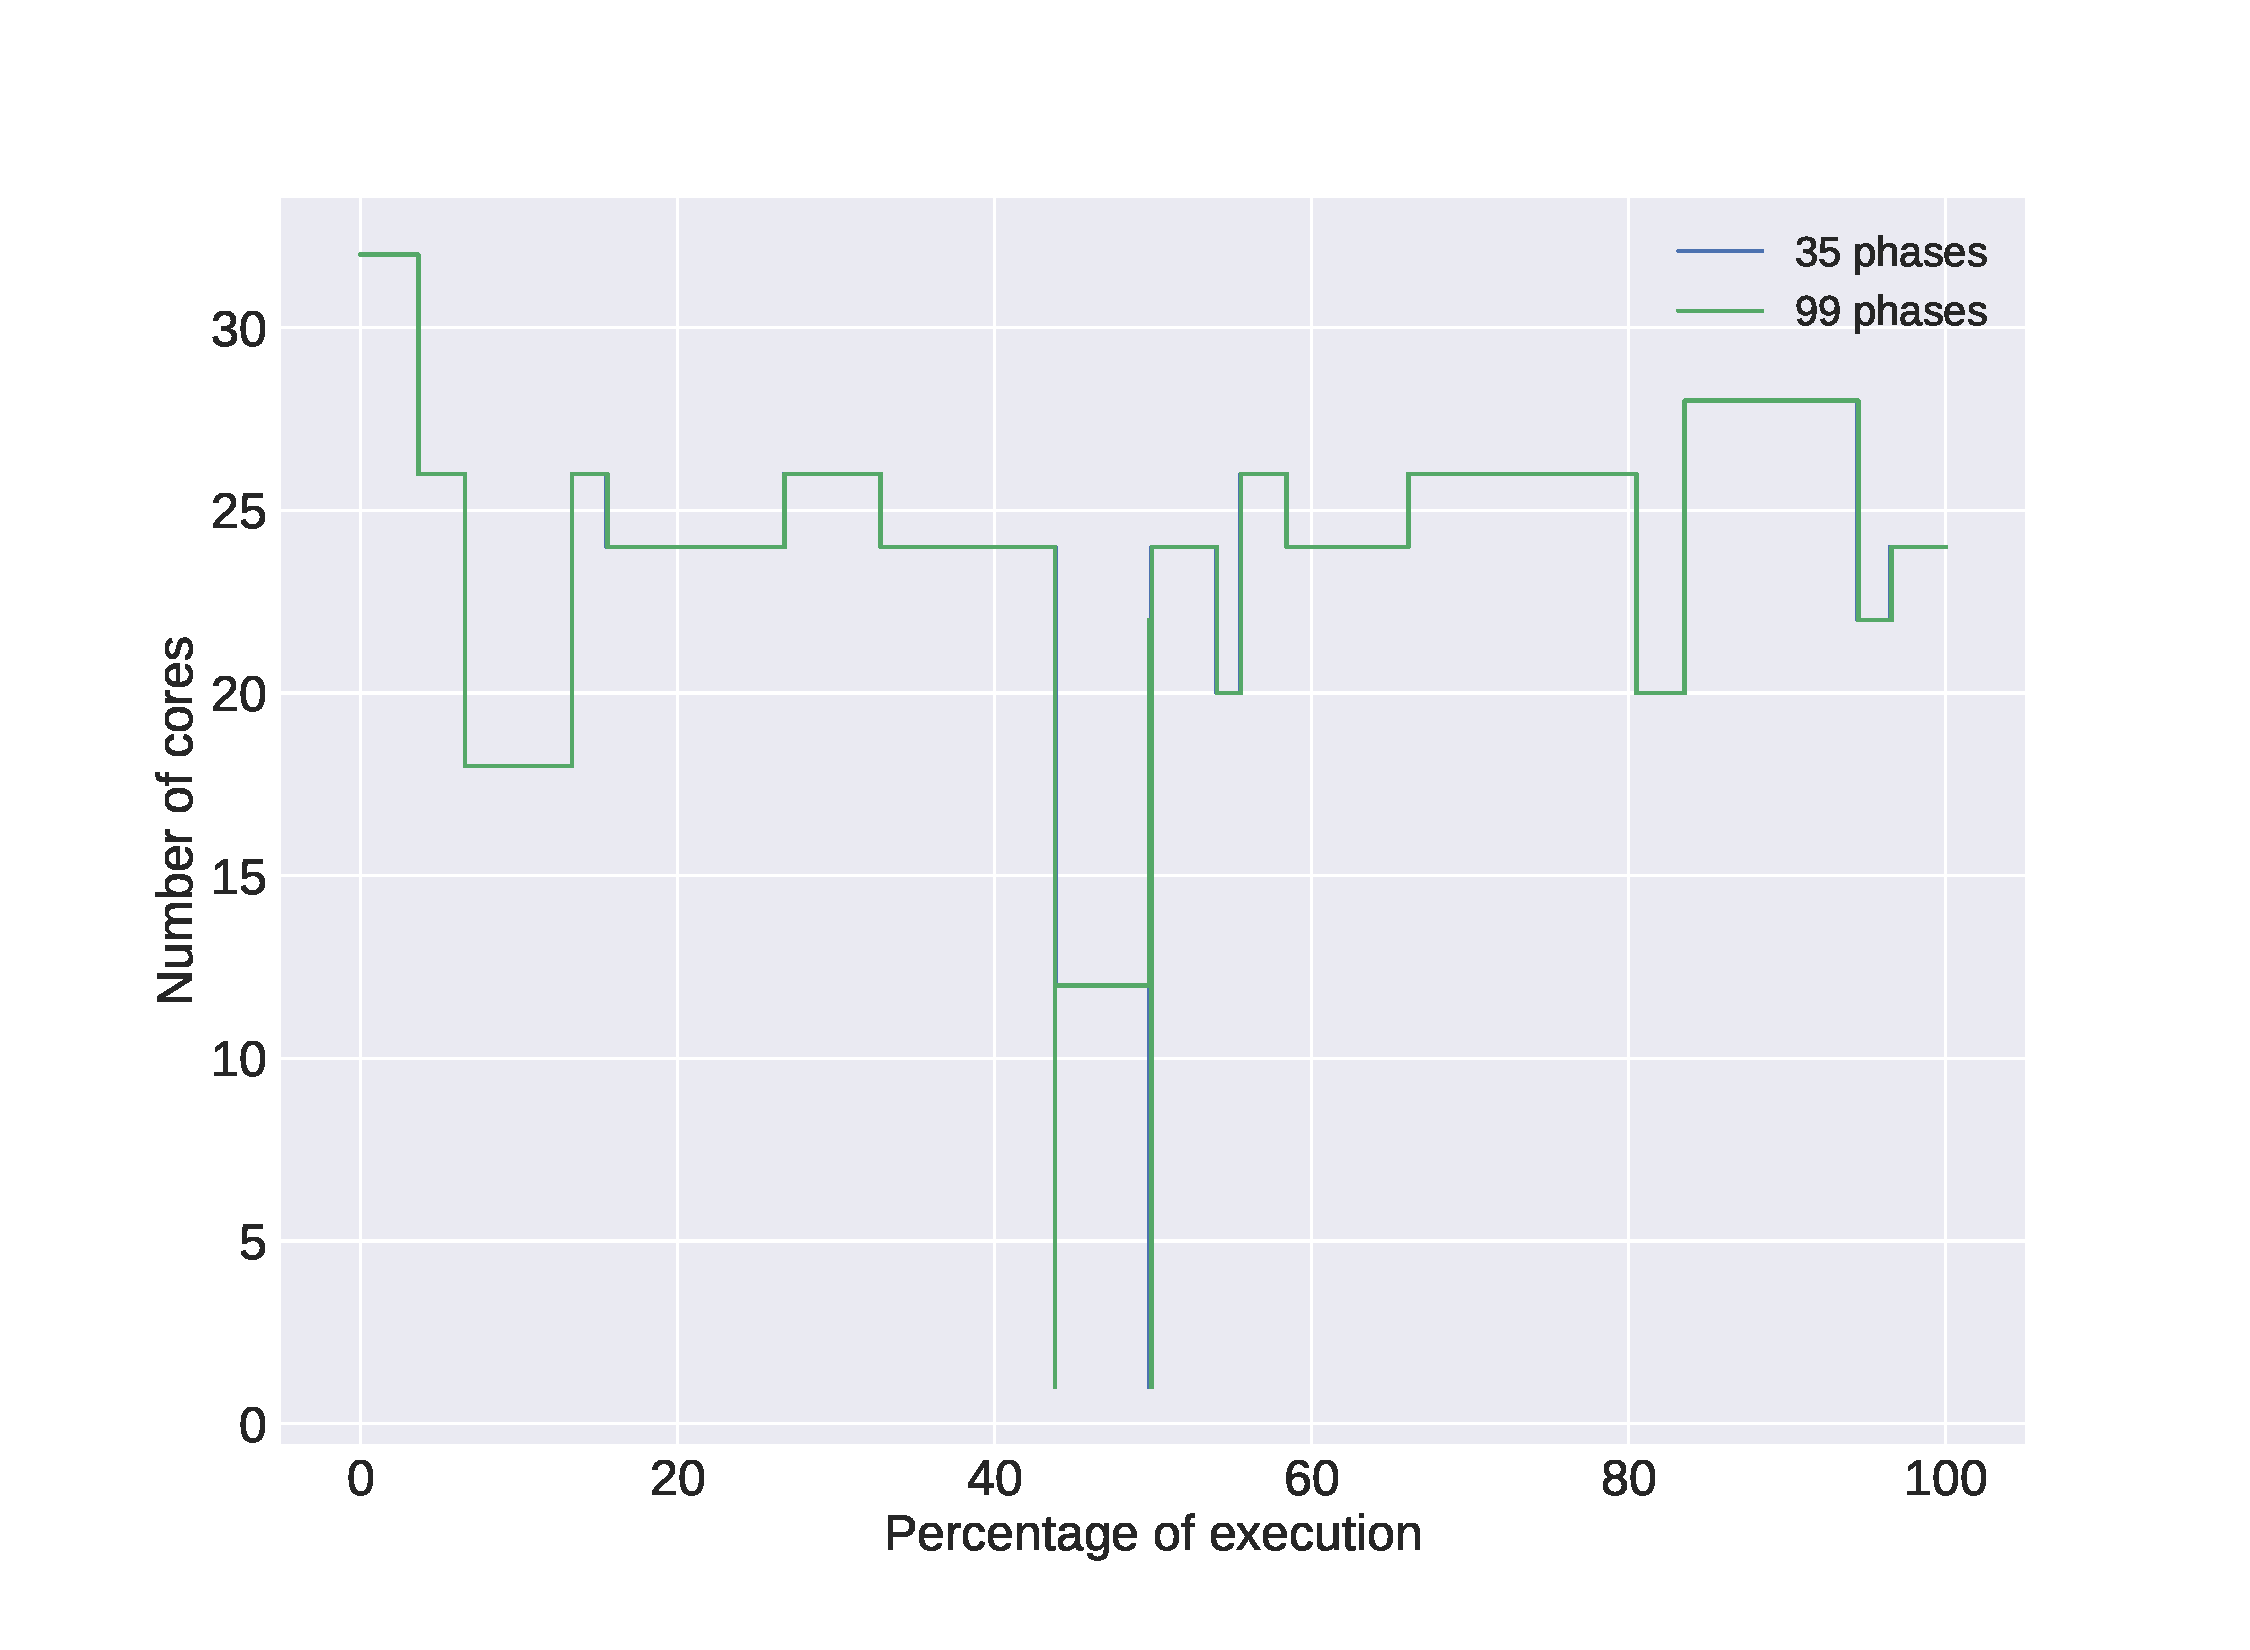
\includegraphics[width=\columnwidth]{phases/figures/signals/completo_bodytrack_1_cores_signals_cmp.pdf}
	\caption{number of cores vs percentage of execution for the Bodytrack application, comparison when using 35 and 99 phases.}
	\label{fig:cores_control_1}
\end{figure}%
\begin{figure}[h]
	\centering
	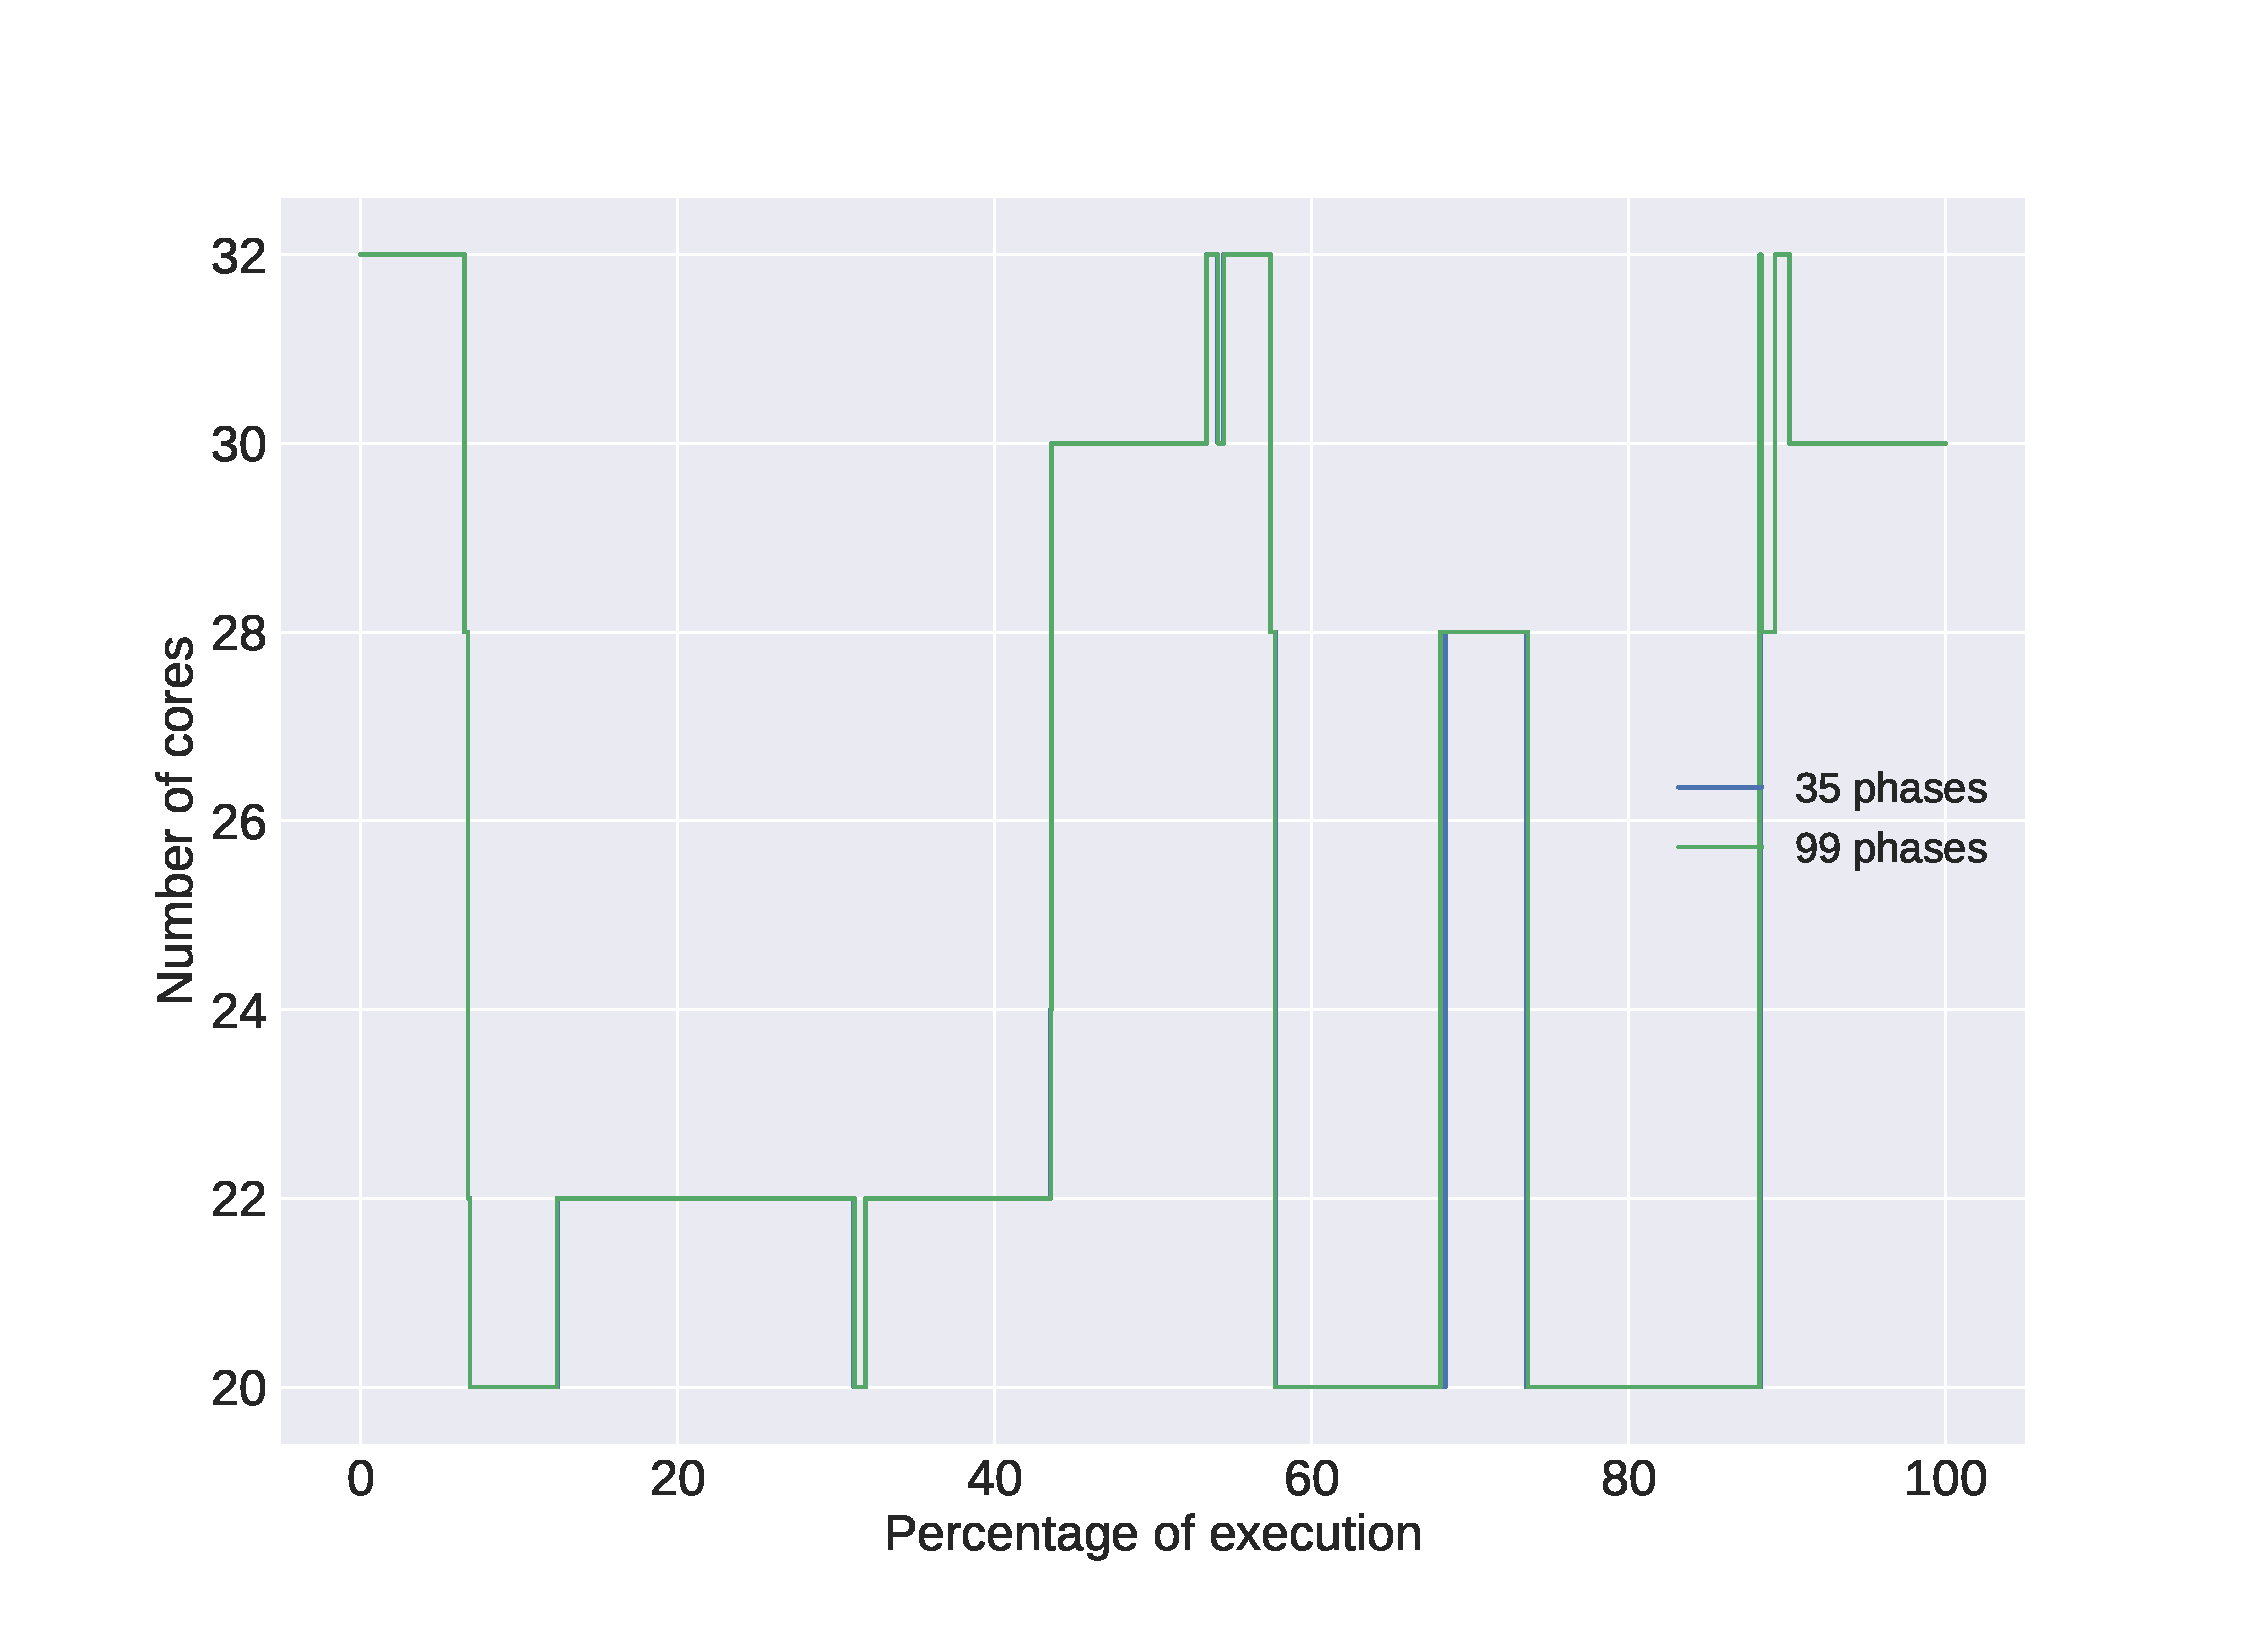
\includegraphics[width=\columnwidth]{phases/figures/signals/completo_black_1_cores_signals_cmp.pdf}
	\caption{number of cores vs percentage of execution for the Blackscholes application, comparison when using 35 and 99 phases.}
	\label{fig:cores_control_2}
\end{figure}%

When we compare this method with the default DVFS algorithm in Linux, we observer an average saving of 38\%, as shown in \cref{fig:cmp_ondemand}, the relative energy per application with different input sizes.

\begin{figure}[H]
	\centering
	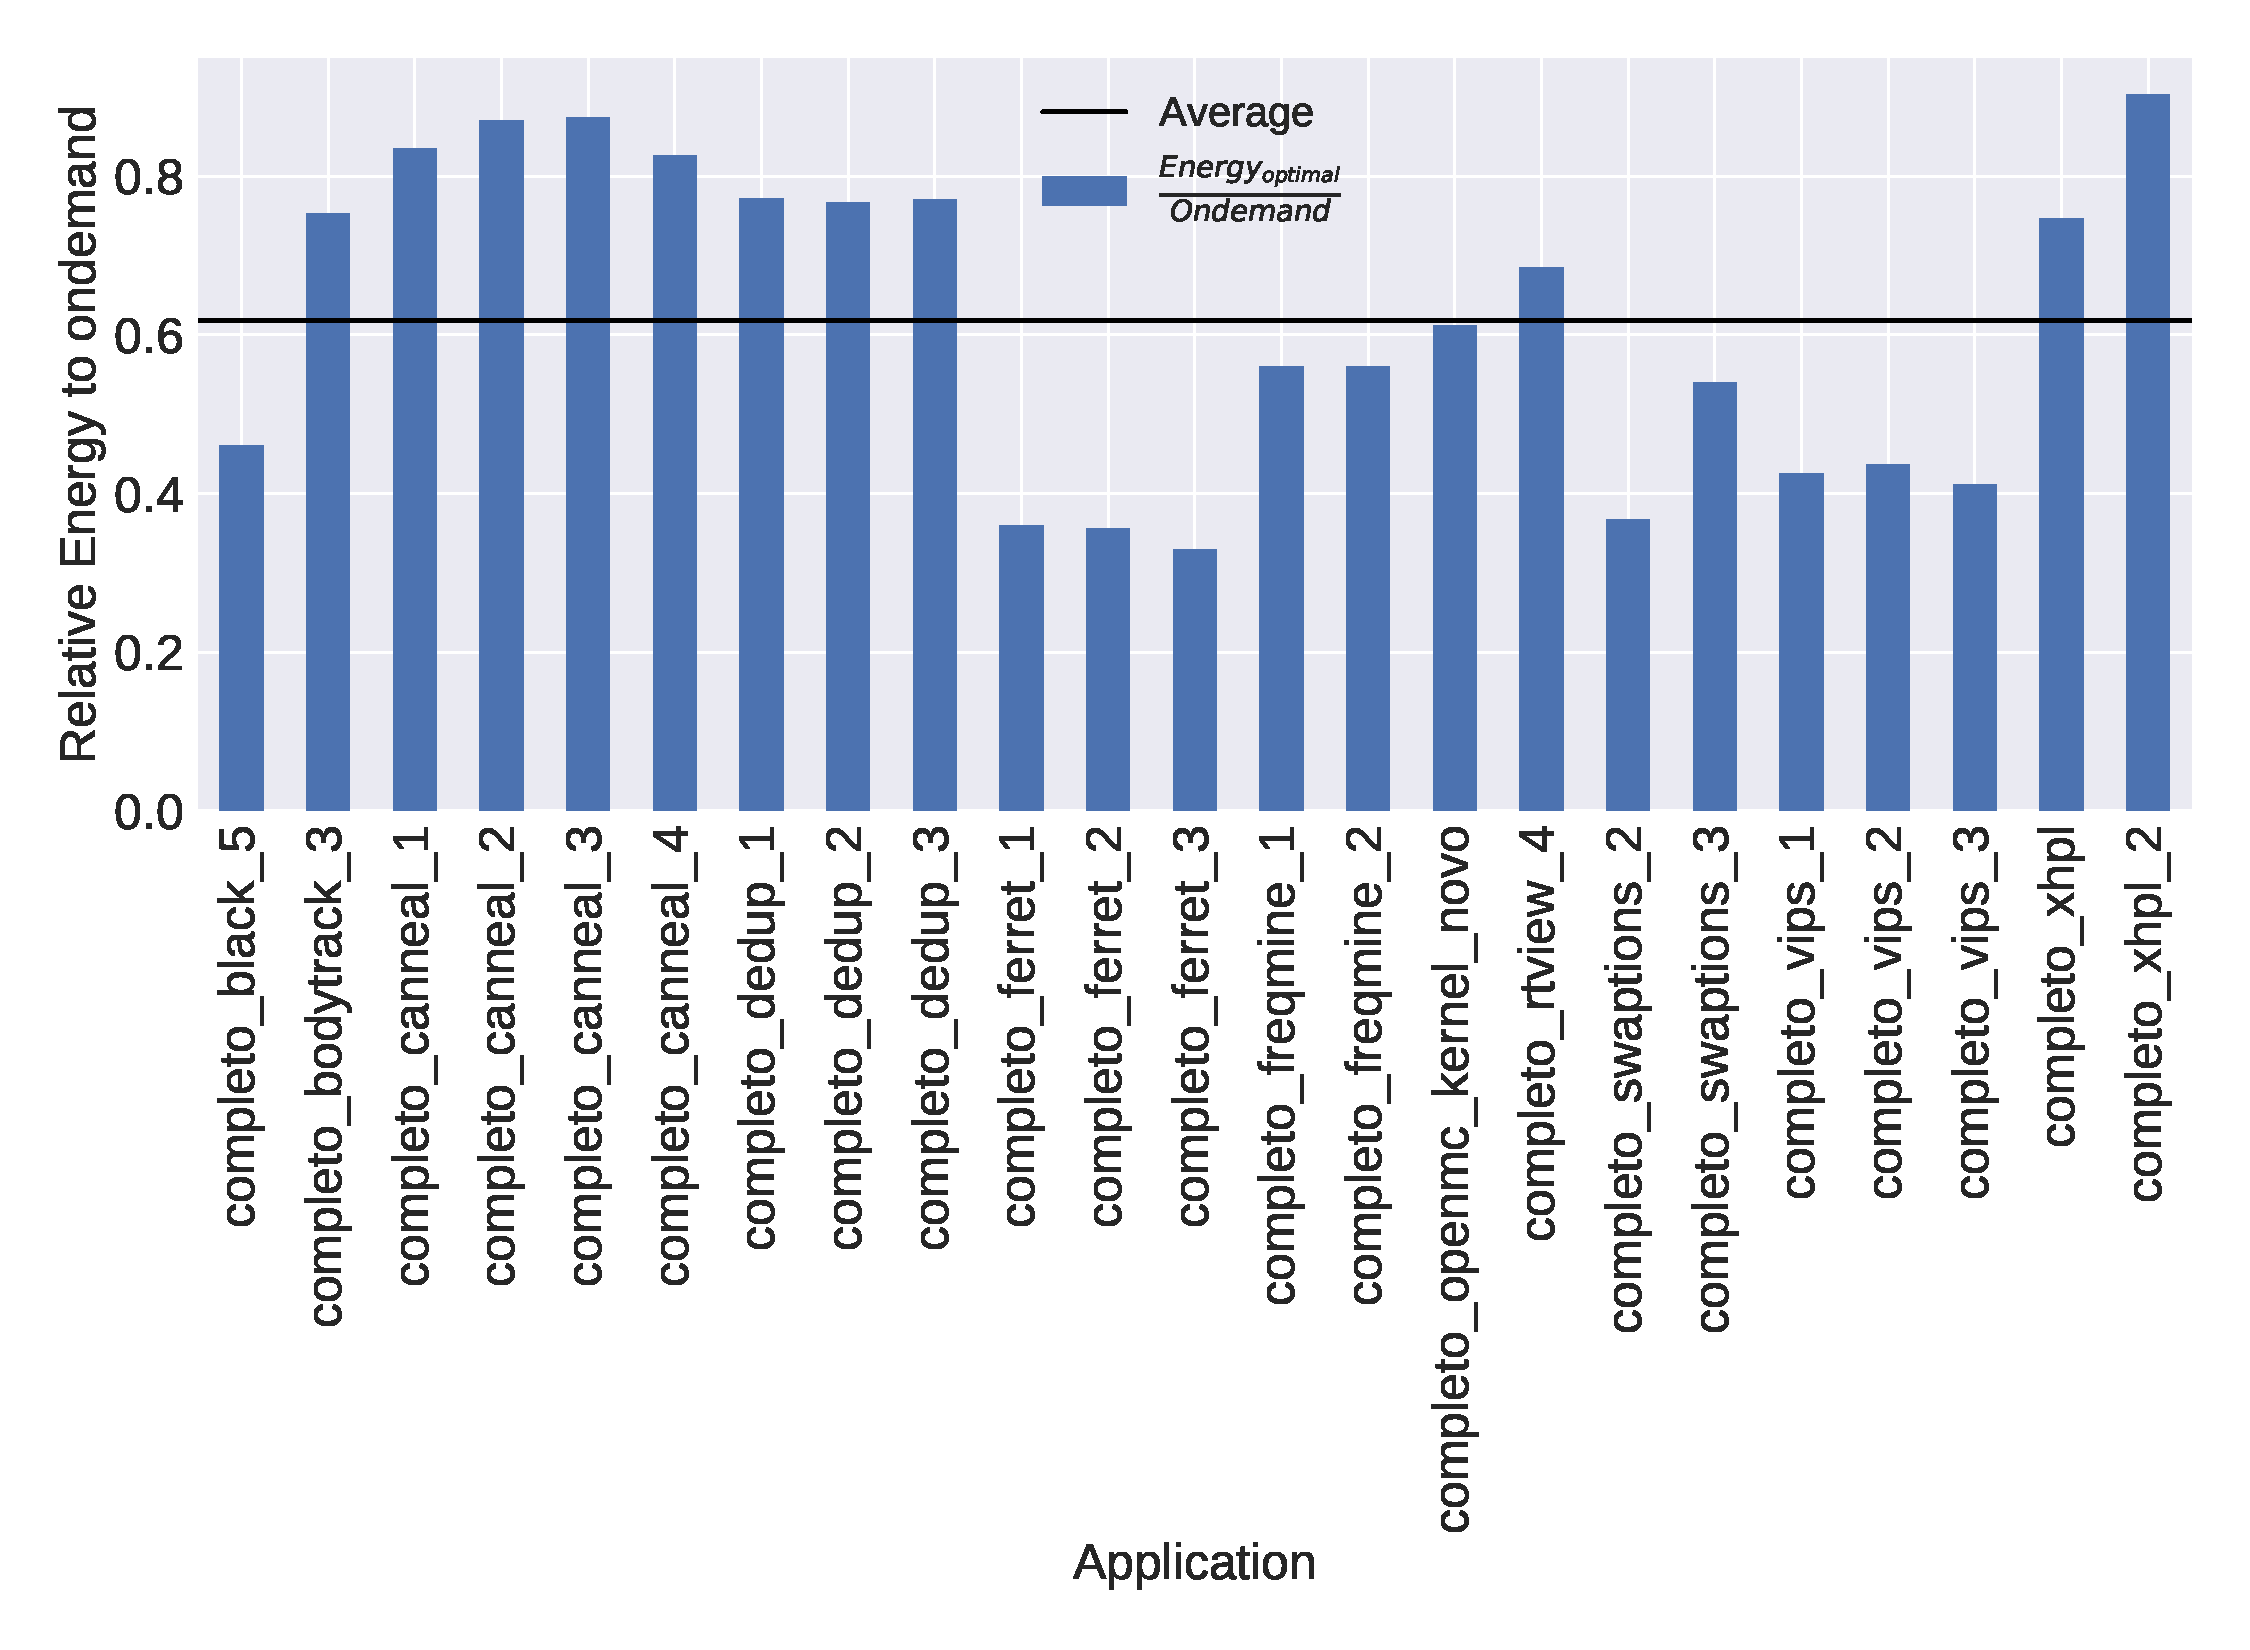
\includegraphics[width=\columnwidth]{phases/figures/comparison_ondemand.pdf}
	\caption{Optimal phase splitting energy vs. on-demand governor on Linux: relative energy comparison for applications with different input sizes.}
	\label{fig:cmp_ondemand}
\end{figure}

To illustrate the phases division, the \cref{fig:phase_division_cmap_3} and \cref{fig:phase_division_cmap_35} show the heatmap for applications when divided with the same number of phases and the percentage of total energy spent in each phase.  The 3 phases division can already show interesting program behavior, such as application setup, loading data, computation and data storage.

\begin{figure}[H]
	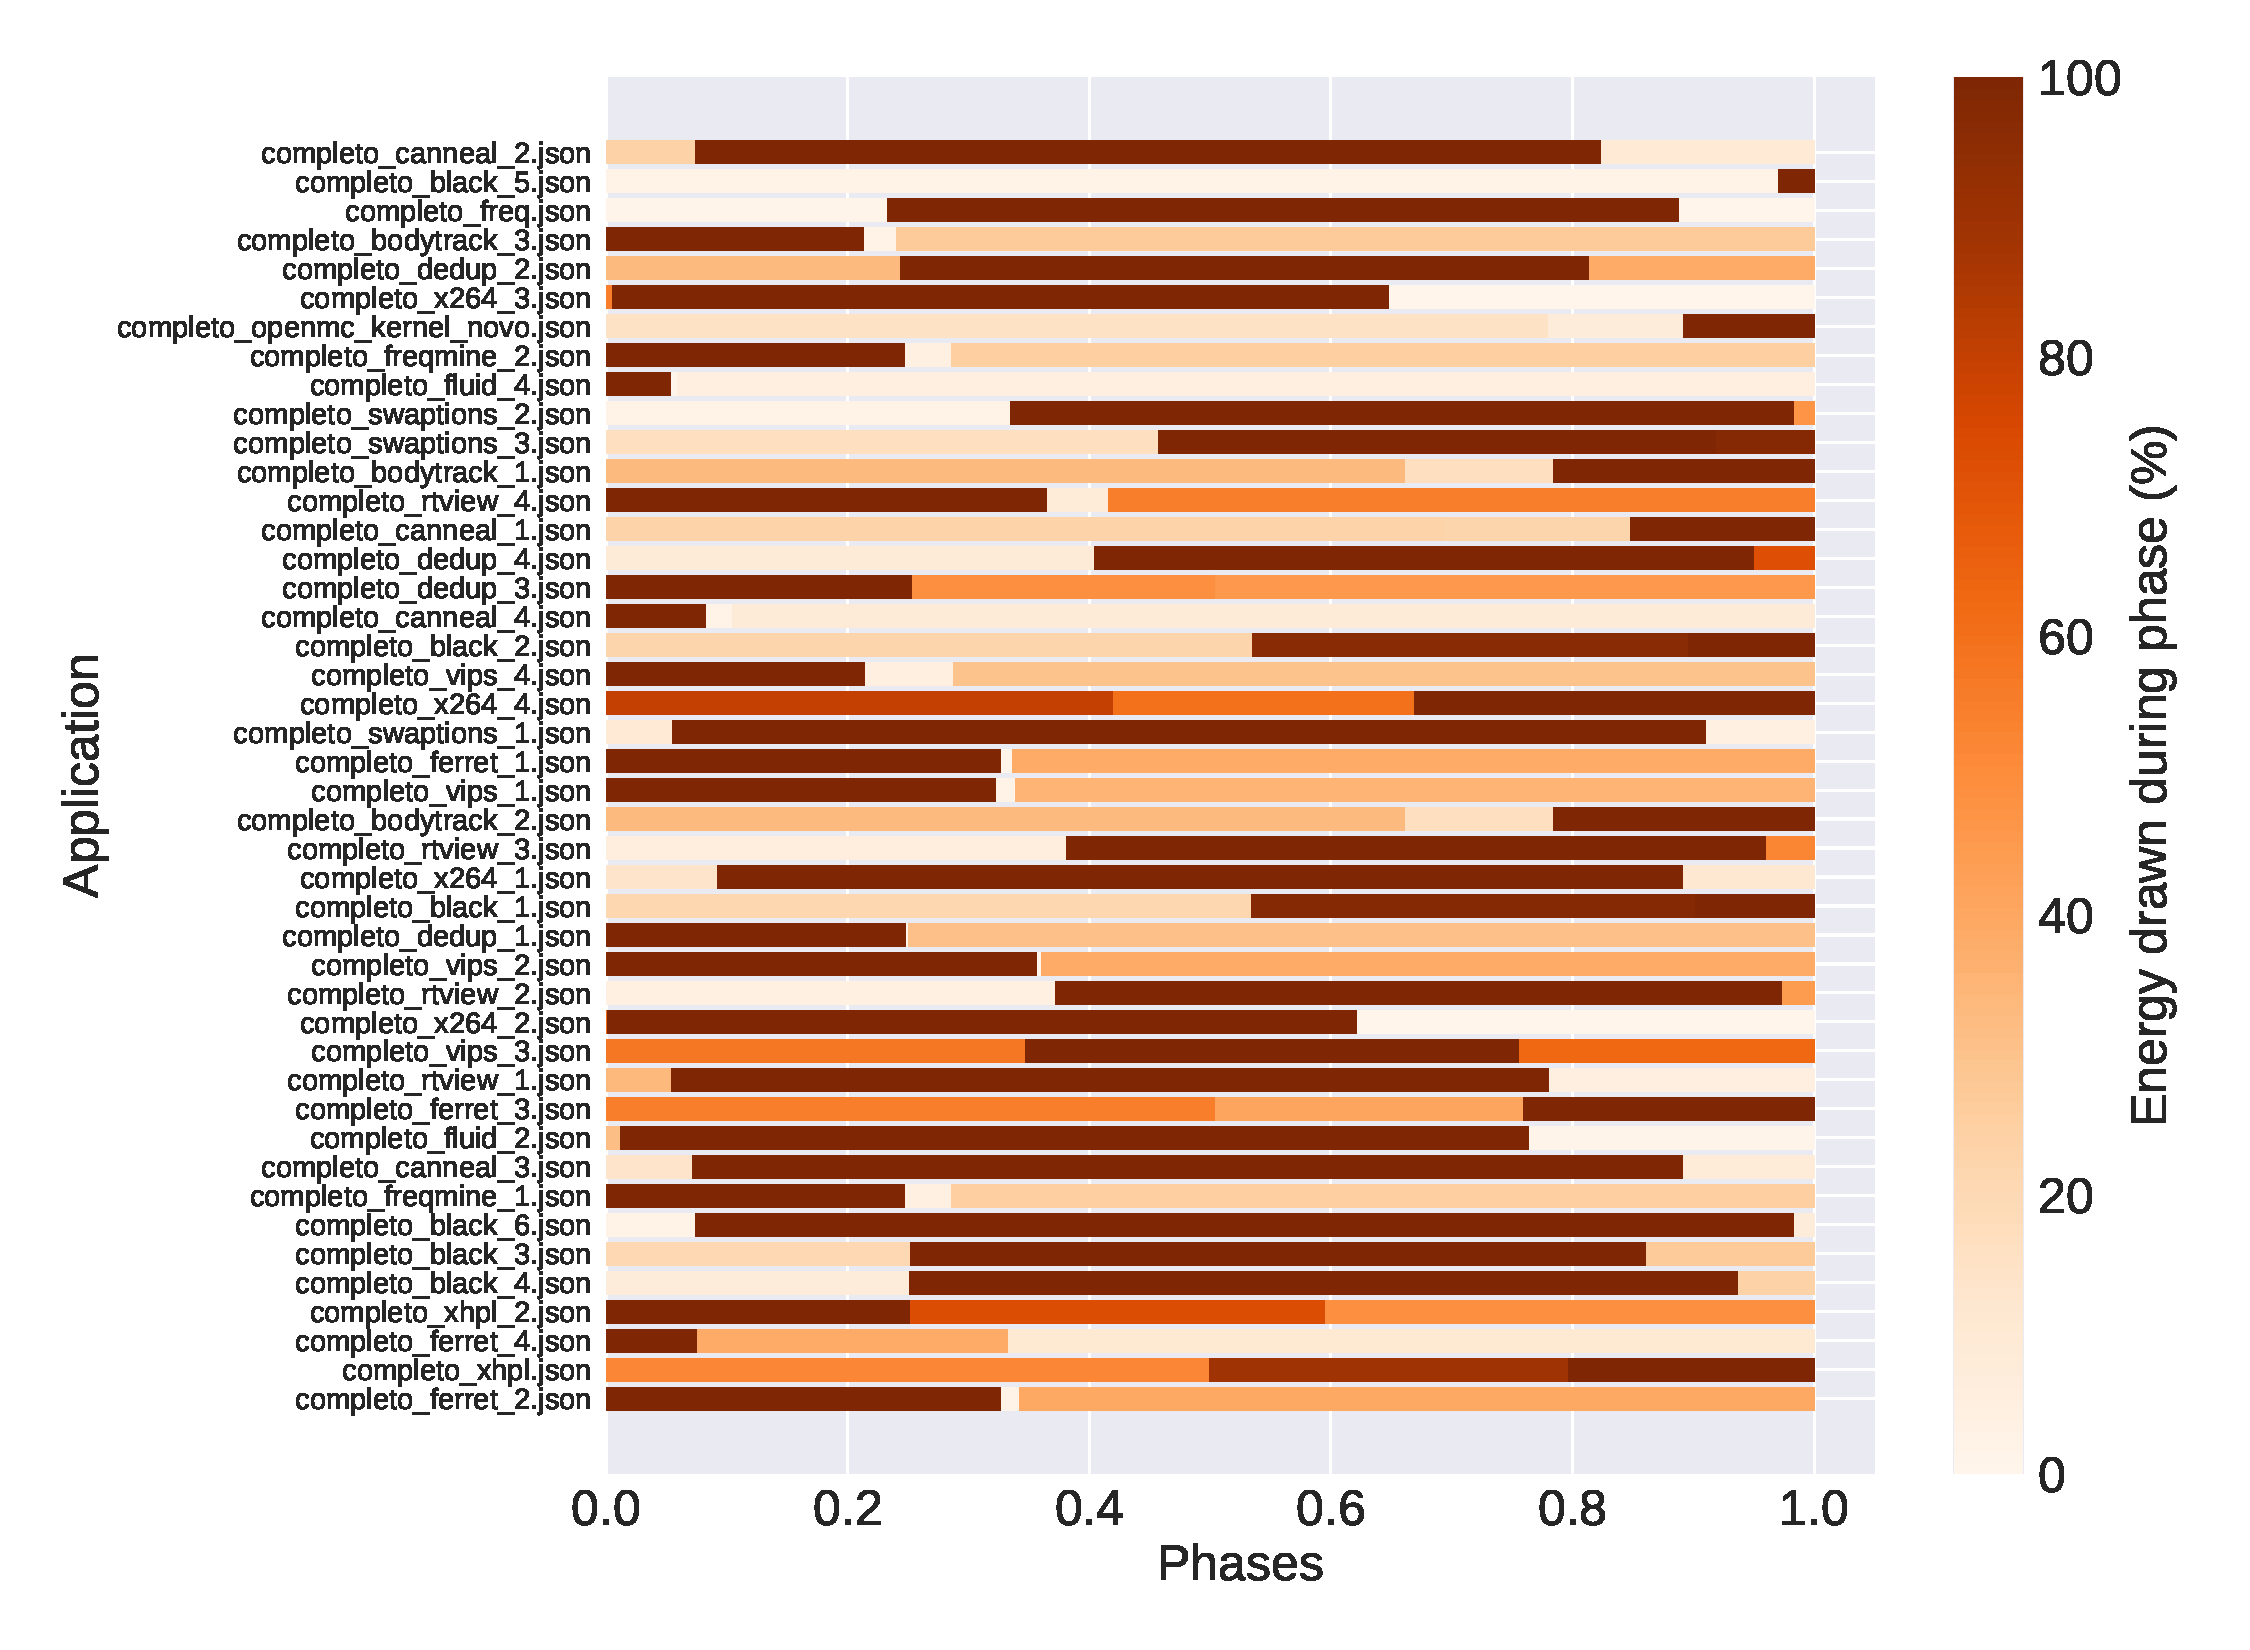
\includegraphics[width=\columnwidth]{phases/figures/phase_division_cmap_3.pdf}
	\caption{Phase division heatmap (3 divisions) showing the energy consumption per phase for all applications.}
	\label{fig:phase_division_cmap_3}
\end{figure}

\begin{figure}[H]
	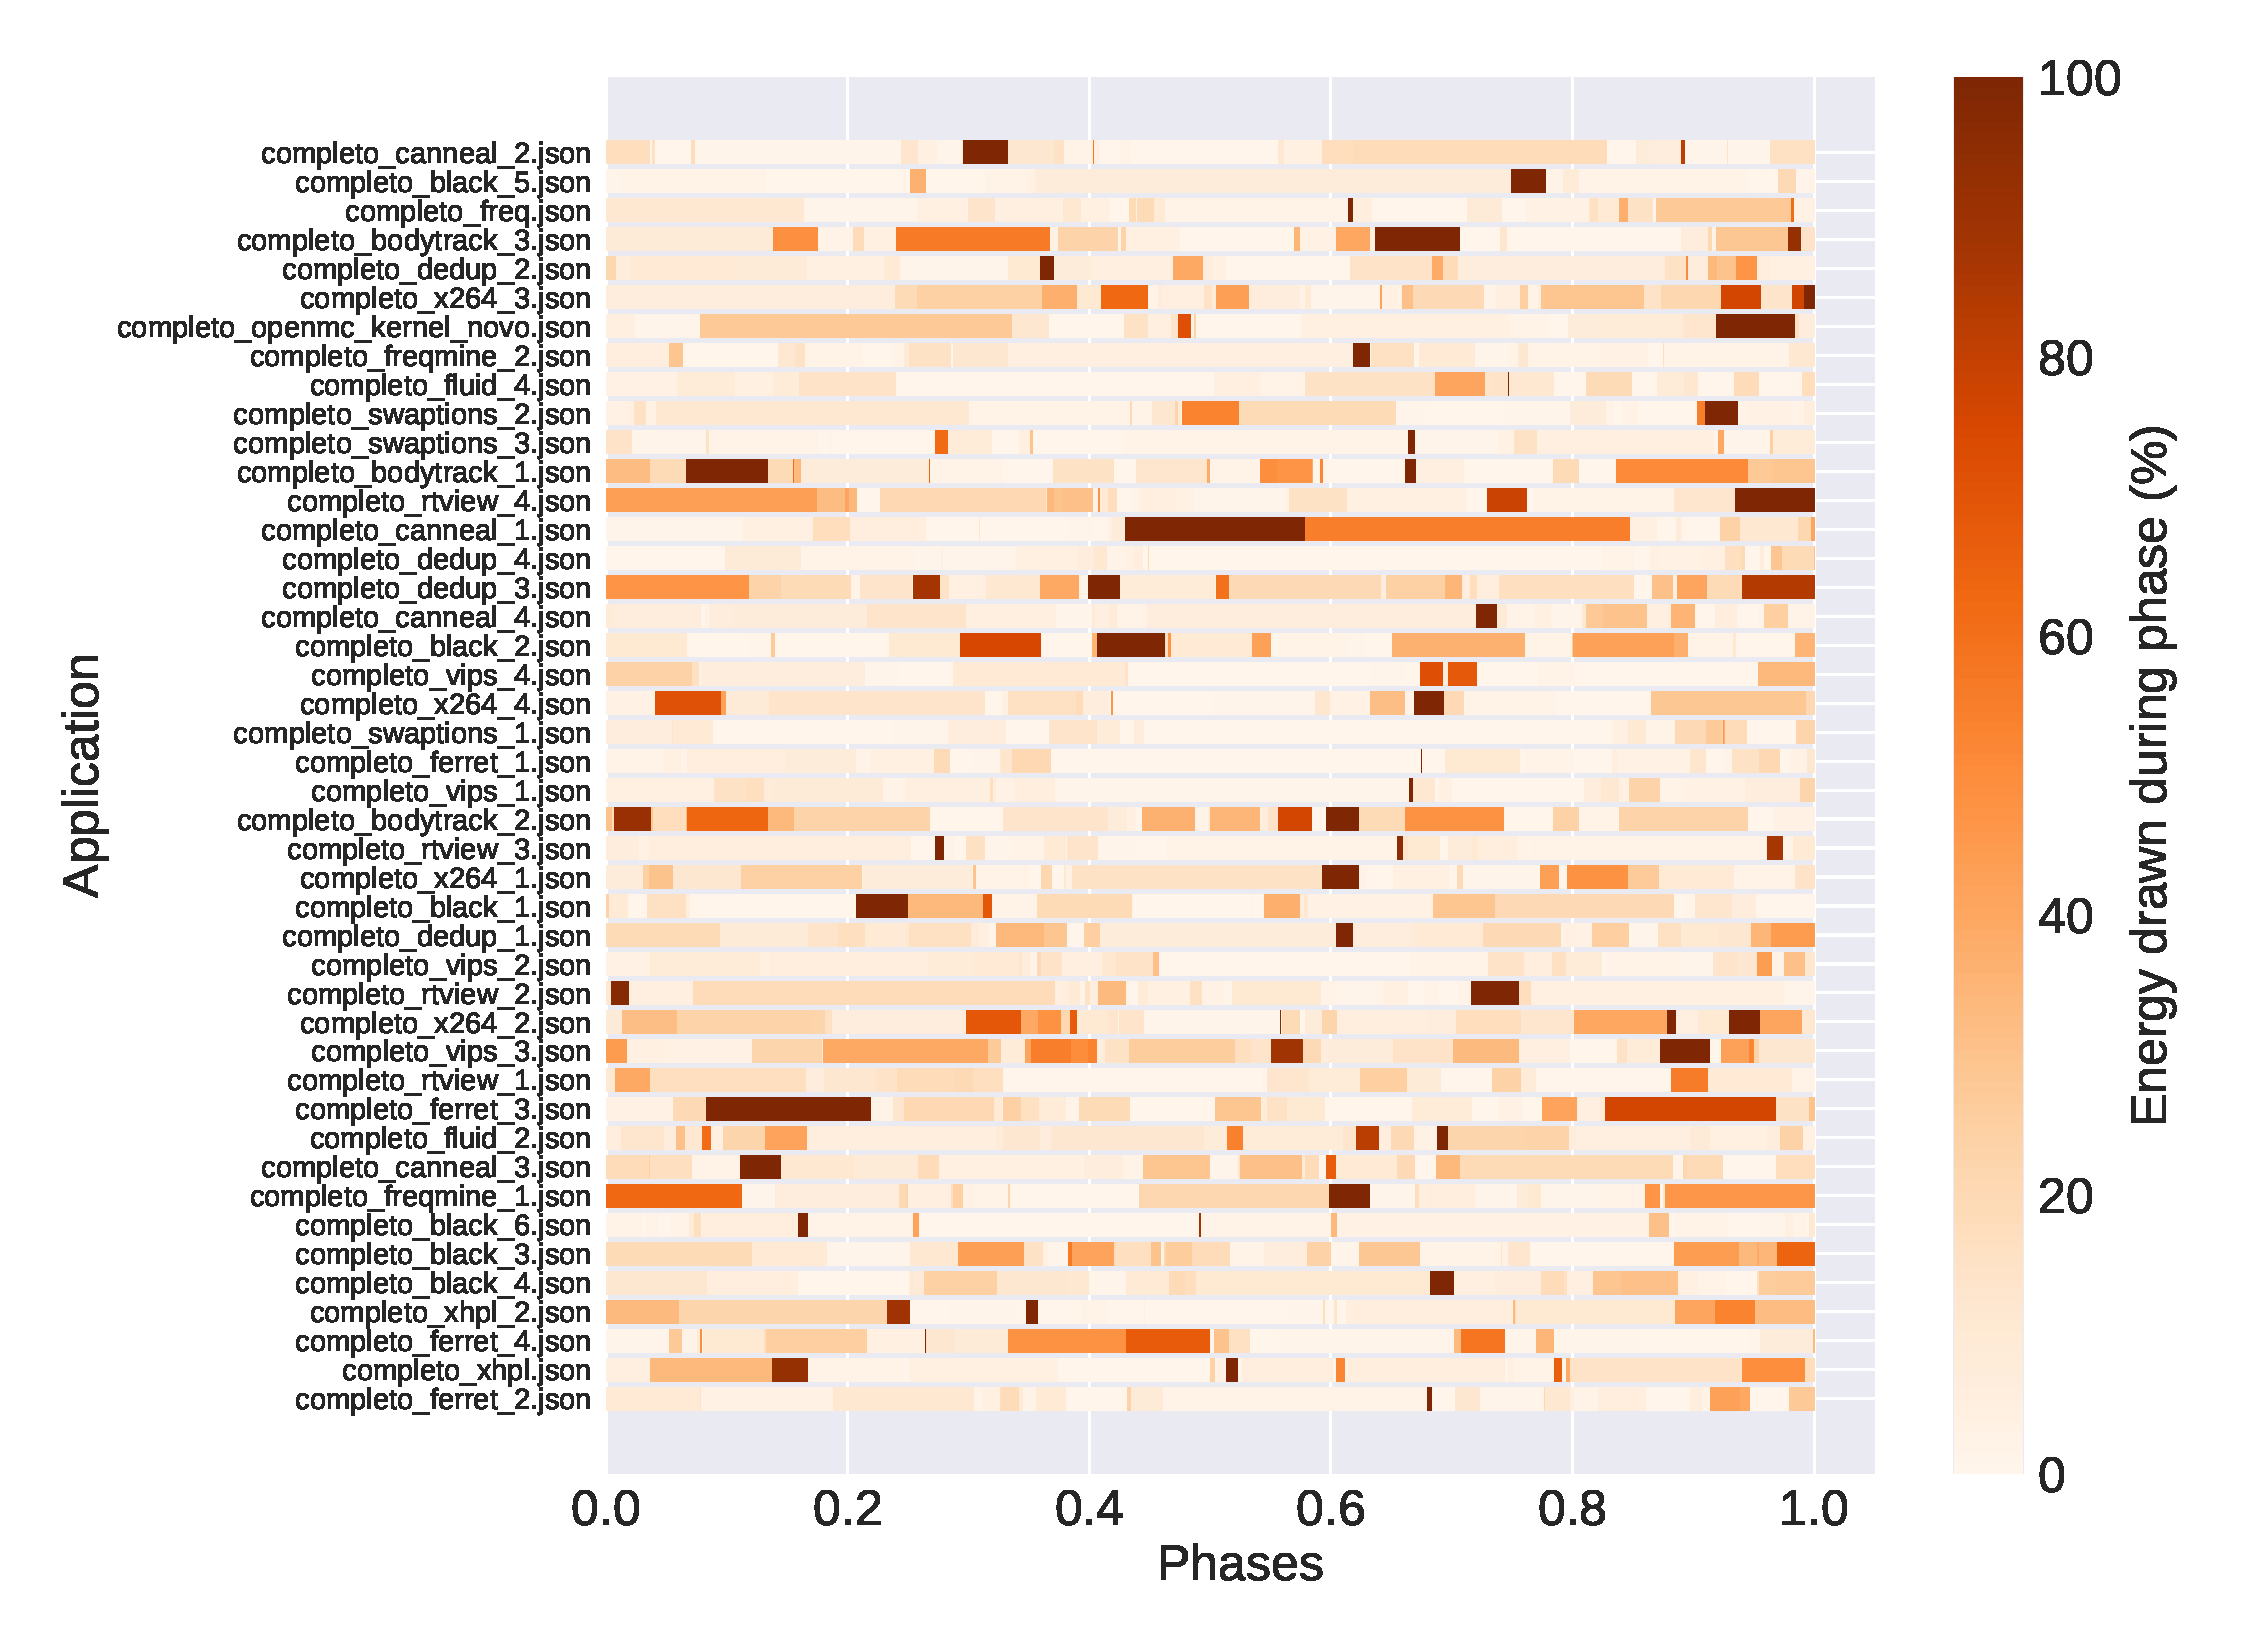
\includegraphics[width=\columnwidth]{phases/figures/phase_division_cmap_35.pdf}
	\caption{Phase division heatmap (35 divisions) showing the energy consumption per phase for all applications.}
	\label{fig:phase_division_cmap_35}
\end{figure}